\section{重积分}

重积分是对多元函数在一个区域上进行积分的过程. 在二维空间中,重积分可以是对平面区域上的函数进行积分; 在三维空间中,重积分可以是对立体区域上的函数进行积分.

\subsection{重积分定义}

\subsubsection{二重积分}

\begin{definition}[二重积分]
    设 $f(x,y)$ 是有界闭区域 $D$ 上的有界函数,将闭区域 $D$ 任意分成 $n$ 个小闭区域 $\Delta\sigma_1,\Delta\sigma_2,\cdots,\Delta\sigma_n$,
    其中 $\Delta\sigma_i$ 表示第 $i$ 个小闭区域,也表示它的面积,在每个 $\Delta\sigma_i$ 上取一点 $(\xi_i,\eta_i)$,
    作乘积 $f(\xi_i,\eta_i)\Delta\sigma_i~~(i=1,2,\cdots,n)$,并作和 $\displaystyle\sum_{i=1}^{n}f(\xi_i,\eta_i)\Delta\sigma_i$,
    如果当各小闭区域的直径中的最大值 $\lambda$ 趋近于零时,这和式极限存在,则称此极限为函数 $f(x,y)$ 在闭区间 $D$ 上的\textit{二重积分},记作
    $\displaystyle\iint\limits_D f(x,y)\dd \sigma$,即 $$ \iint\limits_Df(x,y)\dd\sigma=\lim_{\lambda\to0}\sum_{i=1}^{n}f(\xi_i,\eta_i)\Delta\sigma_i $$
    其中 $\dd \sigma$ 称为面积元.
\end{definition}

\begin{example}
    求 $\displaystyle\lim_{n\to\infty}\dfrac{\pi}{2n^4}\sum_{i=1}^{n}\sum_{j=1}^{n}i^2\sin\dfrac{j\pi}{2n}.$
\end{example}
\begin{solution}
    $\displaystyle\lim_{n\to\infty}\dfrac{\pi}{2n^4}\sum_{i=1}^{n}\sum_{j=1}^{n}i^2\sin\dfrac{j\pi}{2n}=\lim_{n\to\infty}\dfrac{\pi}{2n^2}\sum_{i=1}^{n}\sum_{j=1}^{n}\qty(\dfrac{i}{n})^2\sin\qty(j\dfrac{\pi}{2n})=\int_{0}^{1}x^2\dd x\int_{0}^{\frac{\pi}{2}}\sin y\dd y=\dfrac{1}{3}.$
\end{solution}

\begin{example}[2010 数一]
    计算 $\displaystyle \lim_{n\to\infty}\sum_{i=1}^{n}\sum_{j=1}^{n}\dfrac{n}{(n+i)\qty(n^2+j^2)}.$
\end{example}
\begin{solution}
    由二重积分的定义
    \begin{flalign*}
        I & =\lim_{n\to\infty}\sum_{i=1}^{n}\sum_{j=1}^{n}\dfrac{n}{(n+i)\qty(n^2+j^2)}=\lim_{n\to\infty}\sum_{i=1}^{n}\sum_{j=1}^{n}\dfrac{n}{n\qty(1+\dfrac{i}{n})n^2\qty[1+\qty(\dfrac{j}{n})^2]}              \\
          & =\lim_{n\to\infty}\dfrac{1}{n^2}\sum_{i=1}^{n}\sum_{j=1}^{n}\dfrac{1}{\qty(1+\dfrac{i}{n})\qty[1+\qty(\dfrac{j}{n})^2]}=\int_{0}^{1}\dd x\int_{0}^{1}\dfrac{\dd y}{(1+x)(1+y^2)}=\ln 2\cdot\arctan 1.
    \end{flalign*}
\end{solution}

\begin{example}
    计算极限 $\displaystyle\lim_{n\to\infty}\dfrac{\qty(\sqrt{1}+\sqrt{2}+\cdots+\sqrt{n})\qty(1+\dfrac{1}{\sqrt{2}}+\cdots+\dfrac{1}{\sqrt{n}})}{(n+1)(n+2)}.$
\end{example}
\begin{solution}
    利用二重积分的定义,得
    \begin{flalign*}
        I & =\lim_{n\to\infty}\dfrac{n^2}{(n+1)(n+2)}\dfrac{1}{n}\sum_{k=1}^{n}\sqrt{k}\cdot\dfrac{1}{n}\sum_{k=1}^{n}\dfrac{1}{\sqrt{k}}=\lim_{n\to\infty}\dfrac{n^2}{(n+1)(n+2)}\cdot\lim_{n\to\infty}\dfrac{1}{n}\sum_{k=1}^{n}\sqrt{\dfrac{k}{n}}\cdot\lim_{n\to\infty}\dfrac{1}{n}\sum_{k=1}^{n}\dfrac{1}{\sqrt{\dfrac{k}{n}}} \\
          & =\int_{0}^{1}\sqrt{x}\dd x\cdot\int_{0}^{1}\dfrac{1}{\sqrt{x}}\dd x=\dfrac{2}{3}\cdot2=\dfrac{4}{3}.
    \end{flalign*}
\end{solution}

\subsubsection{三重积分}

\begin{definition}[三重积分]
    设 $ f(x,y,z) $ 是空间闭区域 $\Omega$ 上的有界函数,将 $ \Omega $ 任意分成 $n$ 个小区域 $\Delta v_1,\Delta v_2,\cdots,\Delta v_n$,
    其中 $\Delta v_i$ 表示第 $i$ 个小区域,也表示它的体积,在每个 $\Delta v_i$ 上取一点 $(\xi_i,\eta_i,\zeta _i)$,
    作乘积 $f(\xi_i,\eta_i,\zeta _i)\Delta v_i~~(i=1,2,\cdots,n)$,并作和 $\displaystyle\sum_{i=1}^{n}f(\xi_i,\eta_i,\zeta _i)\Delta v_i$,
    如果当各小区域的直径中的最大值 $\lambda$ 趋近于零时,这和式极限存在,则称此极限为函数 $f(x,y,z)$ 在闭区间 $\Omega$ 上的\textit{三重积分},记作
    $\displaystyle\iiint\limits_\Omega f(x,y,z)\dd v$,即 $$ \iiint\limits_\Omega f(x,y,z)\dd v=\lim_{\lambda\to0}\sum_{i=1}^{n}f(\xi_i,\eta_i,\zeta _i)\Delta v_i $$
    其中 $\dd v$ 称为体积元.
\end{definition}

\begin{example}
    求极限 $\displaystyle\lim_{n\to\infty}\dfrac{\pi}{2n^5}\sum_{i=1}^{n}\sum_{j=1}^{n}\sum_{k=1}^{n}i^2\sin\dfrac{\pi j}{2n}\cos \dfrac{k}{n}.$
\end{example}
\begin{solution}
    $\displaystyle \lim_{n\to\infty}\dfrac{\pi}{2n^3}\sum_{i=1}^{n}\sum_{j=1}^{n}\sum_{k=1}^{n}\qty(\dfrac{i}{n})^2\sin\dfrac{\pi j}{2n}\cos \dfrac{k}{n}=\dfrac{\pi}{2}\int_{0}^{1}x^2\dd x\int_{0}^{1}\sin\qty(\dfrac{\pi}{2}y)\dd y\int_{0}^{1}\cos z\dd z=\dfrac{\pi}{2}\cdot\dfrac{2}{3\pi}\cdot\sin 1=\dfrac{\sin 1}{3}.$
\end{solution}

\subsubsection{重积分大小的比较}

比较二重积分的大小,本质上涉及用二重积分的不等式性质和函数的单调性进行分析讨论.

\begin{example}[2005 数一]
    设 $\displaystyle I_1=\iint\limits_D\cos\sqrt{x^2+y^2}\dd \sigma,~I_2=\iint\limits_D\cos\qty(x^2+y^2)\dd \sigma,~I_3=\iint\limits_D \cos\qty(x^2+y^2)^2\dd \sigma$,其中 $D=\qty{(x,y)\big| x^2+y^2\leqslant 1}$,则
    \begin{tasks}(4)
        \task $I_3>I_2>I_1$
        \task $I_1>I_2>I_3$
        \task $I_2>I_1>I_3$
        \task $I_3>I_1>I_2$
    \end{tasks}
\end{example}
\begin{solution}
    在区域 $D=\qty{(x,y)\big| x^2+y^2\leqslant 1}$ 上有 $0\leqslant x^2+y^2\leqslant 1$,从而有
    $$0\leqslant \qty(x^2+y^2)^2\leqslant x^2+y^2\leqslant \sqrt{x^2+y^2}\leqslant 1<\dfrac{\pi}{2}$$
    又因为 $\cos x$ 在 $\qty(0,\dfrac{\pi}{2})$ 上为单调递减函数,于是
    $$0\leqslant \cos\sqrt{x^2+y^2}\leqslant \cos\qty(x^2+y^2)\leqslant \cos\qty(x^2+y^2)^2$$
    于是 $I_3>I_2>I_1$,选 A.
\end{solution}

\begin{example}
    设区域 $D=\qty{(x,y)\mid (x-1)^2+(y-1)^2\leqslant 2},I_1=\displaystyle\iint\limits_D (x+y)\dd \sigma,I_2=\iint\limits_D\sin(x+y)\dd \sigma$,则下列结论正确的是
    \begin{tasks}(4)
        \task $8\pi>I_1>I_2$
        \task $8\pi\geqslant I_1\geqslant I_2$
        \task $I_1>8\pi>I_2$
        \task $I_1\geqslant 8\pi\geqslant I_2$
    \end{tasks}
\end{example}
\begin{solution}
    作出积分区域后可分析 $x+y$ 的取值范围,\\
    \begin{minipage}{0.29\linewidth}
        \begin{figure}[H]
            \centering
            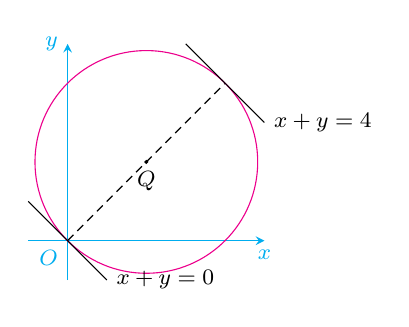
\begin{tikzpicture}[->,samples=100,>=stealth,font=\footnotesize]
                \draw[->,cyan](-.5,0)--(0,0)node[below left]{$O$}--(2.5,0)node[below]{$x$};
                \draw[->,cyan](0,-.5)--(0,2.5)node[left]{$y$};
                \draw[densely dashed,-] (0,0)--(1,1)node[below]{$Q$}--(2,2);
                \draw[fill=black] (1,1) circle(0.5pt);
                \draw[magenta,-] (1,1) circle({sqrt(2)});
                \draw[-,domain=-0.5:0.5,black] plot(\x,{-\x})node[right]{$x+y=0$};
                \draw[-,domain=1.5:2.5,black] plot(\x,{-\x+4})node[right]{$x+y=4$};
            \end{tikzpicture}
            \caption{}
            \label{tikz_ercjf}
        \end{figure}
    \end{minipage}\hfill
    \begin{minipage}{0.7\linewidth}
        由图 \ref{tikz_ercjf} 易知,$0\leqslant x+y\leqslant 4$,所以 $x+y\geqslant \sin(x+y)$,但取等的条件为 $(x,y)=(0,0)$,而在该点出的二重积分为 0,因此
        $$\displaystyle\iint\limits_D(x+y)\dd \sigma>\iint\limits_D\sin(x+y)\dd \sigma$$
        排除 B、D 选项,又因为当 $x+y=4$ 时,有
        $$4\iint\limits_D\dd \sigma=8\pi$$ 并且同样地在 $(2,2)$ 点处的二重积分为 $0$,因此 $8\pi>I_1$,故选 A.
    \end{minipage}
\end{solution}

\begin{example}
    设 $\displaystyle I_1=\iint\limits_D\dfrac{x+y}{4}\dd x\dd y,~I_2=\iint\limits_D\sqrt{\dfrac{x+y}{4}}\dd x\dd y,~I_3=\iint\limits_D\sqrt[3]{\dfrac{x+y}{4}}\dd x\dd y$,
    且 $$D=\qty{(x,y)\big| (x-1)^2+(y-1)^2\leqslant 2}$$
    则有
    \begin{tasks}(4)
        \task $I_1<I_2<I_3$
        \task $I_2<I_3<I_1$
        \task $I_3<I_1<I_2$
        \task $I_3<I_2<I_1$
    \end{tasks}
\end{example}
\begin{solution}
    由图 \ref{tikz_ercjf} 知,$0<\dfrac{x+y}{4}<1$,且 $\dfrac{x+y}{4}<\sqrt{\dfrac{x+y}{4}}<\sqrt[3]{\dfrac{x+y}{4}}$,因此 $I_1<I_2<I_3$,选 A.
\end{solution}

\begin{example}[2019 数二]
    已知平面区域 $D=\qty{(x,y)\Big| |x|+|y|\leqslant\dfrac{\pi}{2}}$,记 $\displaystyle I_1=\iint\limits_D\sqrt{x^2+y^2}\dd x\dd y,~I_2=\iint\limits_D\sin\sqrt{x^2+y^2}\dd x\dd y,~I_3=\iint\limits_D\qty(1-\cos\sqrt{x^2+y^2})\dd x\dd y$,则
    \begin{tasks}(4)
        \task $I_3<I_2<I_1$
        \task $I_2<I_1<I_3$
        \task $I_1<I_2<I_3$
        \task $I_2<I_3<I_1$
    \end{tasks}
\end{example}
\begin{solution}
    作出积分区域 $D$:\\
    \begin{minipage}{0.29\linewidth}
        \begin{figure}[H]
            \centering
            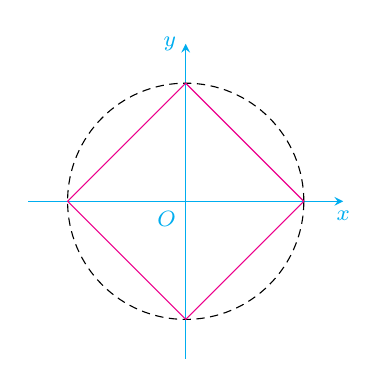
\begin{tikzpicture}[->,samples=100,>=stealth,font=\footnotesize]
                \draw[->,cyan](-2,0)--(0,0)node[below left]{$O$}--(2,0)node[below]{$x$};
                \draw[->,cyan](0,-2)--(0,2)node[left]{$y$};
                % \draw[densely dashed,-] (0,0)--(1,1)node[below]{$Q$}--(2,2);
                % \draw[fill=black, densely dashed] (0,0) circle(0.5pt);
                \draw[densely dashed] (0,0) circle(1.5);
                \draw[-,magenta] (1.5,0)--(0,1.5)--(-1.5,0)--(0,-1.5)--(1.5,0);
                % \draw[-,domain=-0.5:0.5,black] plot(\x,{-\x})node[right]{$x+y=0$};
                % \draw[-,domain=1.5:2.5,black] plot(\x,{-\x+4})node[right]{$x+y=4$};
            \end{tikzpicture}
            \caption{}
            \label{tikz_ercjfshuer}
        \end{figure}
    \end{minipage}\hfill
    \begin{minipage}{0.7\linewidth}
        在区域 $D$ 上,有 $0\leqslant \sqrt{x^2+y^2}\leqslant \dfrac{\pi}{2}$,那么 $$\sin\sqrt{x^2+y^2}\leqslant \sqrt{x^2+y^2}$$
        下面比较 $1-\cos\sqrt{x^2+y^2}$ 与 $\sin\sqrt{x^2+y^2}$,令 $u=\sqrt{x^2+y^2}\in\qty[0,\dfrac{\pi}{2}]$,那么
        $$1-\cos\sqrt{x^2+y^2}-\sin\sqrt{x^2+y^2}=1-\cos u-\sin u=1-\sqrt{2}\sin\qty(u+\dfrac{\pi}{4})\leqslant 0$$
        故 $1-\cos\sqrt{x^2+y^2}\leqslant \sin\sqrt{x^2+y^2}\leqslant \sqrt{x^2+y^2}$,所以 $I_3<I_2<I_1$,选 A.
    \end{minipage}
\end{solution}
\subsection{重积分的计算及相关方法}

\subsubsection{重积分的性质}

\begin{example}[1993 年数三]
    设 $f(x,y)$ 连续,且
    $$f(x,y)=xy+\iint\limits_D f(u,v)\dd u\dd v$$
    其中 $D$ 是由 $y=0,y=x^2,x=1$ 所围成区域,求 $f(x,y)$.
\end{example}
\begin{solution}
    设 $A=\displaystyle\iint\limits_D f(u,v)\dd u\dd v$,则 $f(x,y)=xy+A$,等式两边分别积分,得
    \begin{flalign*}
        A=\iint\limits_D f(x,y)\dd x\dd y=\iint\limits_D(xy+A)\dd x\dd y=\int_{0}^{1}\dd x\int_{0}^{x^2}(xy+A)\dd y=\int_{0}^{1}\qty(\dfrac{1}{2}x^5+Ax^2)\dd x=\dfrac{4A+1}{12}
    \end{flalign*}
    即 $A=\dfrac{1}{8}$,于是 $f(x,y)=xy+\dfrac{1}{8}.$
\end{solution}

\begin{example}
    计算二重积分 \(\displaystyle\iint\limits_Dy^2\dd x\dd y\),其中 \(D\) 是由摆线 \(\begin{cases}
        x=a(t-\sin t) \\
        y=a(1-\cos t)
    \end{cases}(0\leqslant t\leqslant 2\pi,a>0)\) 与 \(x\) 轴围成的区域.
\end{example}
\begin{solution}
    因为 $y=a(1-\cos t),~\dd x=a(1-\cos t)\dd t$,于是
    \begin{flalign*}
        \iint\limits_Dy^2\dd x\dd y & =\int_{0}^{2\pi a}\dd x\int_{0}^{y(x)}y^2\dd y=\dfrac{1}{3}\int_{0}^{2\pi a}y^3(x)\dd x=\dfrac{1}{3}\int_{0}^{2\pi}a^4(1-\cos t)^4\dd t=\dfrac{a^4}{3}\int_{0}^{2\pi}\qty(2\sin^2\dfrac{t}{2})^4\dd t                                                                       \\
                                    & \xlongequal{\frac{t}{2}=u}\dfrac{a^4}{3}\cdot 2^4\cdot 2\int_{0}^{\pi}\sin^8u\dd u=\dfrac{a^4}{3}\cdot 2^6\int_{0}^{\frac{\pi}{2}}\sin^8u\dd u=\dfrac{a^4}{3}\cdot 2^6\cdot\dfrac{1\times3\times5\times7}{2\times4\times6\times8}\cdot\dfrac{\pi}{2}=\dfrac{35\pi}{12} a^4.
    \end{flalign*}
\end{solution}

\begin{example}
    设 \(D\) 由 \(\begin{cases}
        x=t-\sin t \\
        y=1-\cos t
    \end{cases}(0\leqslant t\leqslant 2\pi)\) 与 \(x\) 围成,求 \(\displaystyle\iint\limits_D(x+2y)\dd x\dd y\).
\end{example}
\begin{solution}
    \begin{flalign*}
        I=\iint\limits_D (x+2y)\dd x\dd y=\int_{0}^{2\pi}\dd x\int_{0}^{y(x)}(x+2y)\dd y=\int_{0}^{2\pi}\qty(xy+y^2)\dd x=\int_{0}^{2\pi}\qty[(t-\sin t)(1-\cos t)^2+(1-\cos t)^3]\dd t
    \end{flalign*}
    令 \(\displaystyle I_1=\int_{0}^{2\pi}t(1-\cos t)^2\dd t,~I_2=\int_{0}^{2\pi}\sin t(1-\cos t)^2\dd t,~I_3=\int_{0}^{2\pi}(1-\cos t)^3\dd t\),则
    \begin{flalign*}
        I_1 & =\int_{0}^{2\pi}t\qty(2\sin^2\dfrac{t}{2})^2\dd t \xlongequal{\frac{t}{2}=u}16\int_{0}^{\pi}u\cdot\sin^4u\dd u \xlongequal{\int_{0}^{\pi}x\cdot f(\sin x)\dd x=\frac{\pi}{2}\int_{0}^{\pi}f(\sin x)\dd x}16\pi\cdot\dfrac{1\times3}{2\times4}\cdot\dfrac{\pi}{2}=3\pi^2 \\
        I_3 & =\int_{0}^{2\pi}\qty(2\sin^2\dfrac{t}{2})^3\dd t=8\int_{0}^{2\pi}\sin^6\dfrac{t}{2}\dd t \xlongequal{\frac{t}{2}=u}32\int_{0}^{\frac{\pi}{2}}\sin^6u\dd u=32\times\dfrac{1\times3\times5}{2\times4\times6}\cdot\dfrac{\pi}{2}=5\pi
    \end{flalign*}
    且 \(\displaystyle I_2=\int_{0}^{2\pi}\sin t(1-\cos t)^2\dd t \xlongequal[\text{偶倍奇零}]{u=\pi-t}0 \),故 $I=I_1-I_2+I_3=3\pi ^2+5\pi.$
\end{solution}

\subsubsection{运用分部积分法}

\begin{example}
    计算 $\displaystyle\int_{0}^{1}\dd y\int_{1}^{\sqrt{y}}\sqrt{\dfrac{1}{x^2}+1}\dd x.$
\end{example}
\begin{solution}
    由分部积分公式,
    $$I=\int_{0}^{1}\qty[\int_{1}^{\sqrt{y}}\sqrt{\dfrac{1}{x^2}+1}\dd x]\dd y=\eval{y\int_{1}^{\sqrt{y}}\sqrt{\dfrac{1}{x^2}+1}\dd x}_{y=0}^{y=1}-\int_{0}^{1}y\dd \qty[\int_{1}^{\sqrt{y}}\sqrt{\dfrac{1}{x^2}+1}\dd x]=0-\dfrac{1}{2}\int_{0}^{1}\sqrt{1+y}\dd y=1-2\sqrt{2}.$$
\end{solution}

\begin{example}
    计算二重积分 $\displaystyle I=\int_{0}^{1}\dd x\int_{x-x^3}^{1}\qty(3x^2-1)\e^{y^2}\dd y.$
\end{example}
\begin{solution}
    令 $\varphi(x)=\displaystyle\int_{x-x^3}^{1}\e^{y^2}\dd y$,于是原式可化为
    \begin{flalign*}
        I & =\int_{0}^{1}\qty(3x^2-1)\varphi(x)\dd x=\int_{0}^{1}\varphi(x)\dd \qty(x^3-x)=\qty(x^3-x)\varphi(x)\biggl |_{x=0}^{x=1}-\int_{0}^{1}\qty(x^3-x)\qty(3x^2-1)\e^{\qty(x-x^3)^2}\dd x \\
          & =-\dfrac{1}{2}\int_{0}^{1}\e^{\qty(x-x^3)^2}\dd \qty(x-x^3)^2=-\dfrac{1}{2}\e^{\qty(x-x^3)^2}\biggl |_{x=0}^{x=1}=0.
    \end{flalign*}
\end{solution}

\begin{example}
    计算二重积分 $\displaystyle\int_{0}^{1}\dd x\int_{x^2}^{1}x^3\sin y^3\dd y$.
\end{example}
\begin{solution}
    令 $\varphi(x)=\displaystyle\int_{x^2}^{1}\sin y^3\dd y$,于是原式可化为
    \begin{flalign*}
        I & =\int_{0}^{1}x^3\varphi(x)\dd x=\dfrac{1}{4}\int_{0}^{1}\varphi(x)\dd x^4=\dfrac{1}{4}x^3\varphi(x)\biggl |_{x=0}^{x=1}-\dfrac{1}{4}\int_{0}^{1}x^4\cdot\qty(-2x\sin x^6)\dd x \\
          & =\dfrac{1}{2}\int_{0}^{1}x^5\sin x^6\dd x=\dfrac{1}{12}\int_{0}^{1}\sin x^6\dd x^6=\eval{\dfrac{-\cos x^6}{12}}_{x=0}^{x=1}=\dfrac{1-\cos 1}{12}.
    \end{flalign*}
\end{solution}

\subsubsection{交换积分顺序}

\begin{example}[2004 数一]
    设 $f(x)$ 为连续函数,$\displaystyle F(t)=\int_{0}^{t}\dd y\int_{y}^{t}f(x)\dd x$,则 $F'(2)$ 等于
    \begin{tasks}(4)
        \task $2f(2).$
        \task $f(2).$
        \task $-f(2).$
        \task $0.$
    \end{tasks}
\end{example}
\begin{solution}
    交换积分次序,$\displaystyle F(t)=\int_{1}^{t}\dd x\int_{1}^{x}f(x)\dd y=\int_{1}^{t}(x-1)f(x)\dd x$,
    于是 $F'(2)=(2-1)f(2)=f(2)$,故选 B.
\end{solution}

% \begin{example}
%     (2015 数学 (一)、(二))计算 $\displaystyle\iint\limits_Dx(x+y)\dd x\dd y$,其中 $D=\{(x,y)|x^2+y^2\leqslant 2,y\geqslant x^2\}.$
% \end{example}
% \begin{solution}
%     因为区域 $D$ 关于 $y$ 轴对称,所以
%     \begin{flalign*}
%         \iint\limits_Dx(x+y)\dd x\dd y
%          & =2\int_0^1\dd x\int_{x^2}^{\sqrt{2-x^2}}x^2\dd y
%         =2\int_0^1\left(x^2\sqrt{2-x^2}-x^4\right)\dd x                                        \\
%          & =2\int_0^1x^2\sqrt{2-x^2}\dd x-\frac{2}{5}
%         \xlongequal[]{x=\sqrt{2}\sin t}2\int_0^{\frac{\pi}{4}}4\sin^2t\cos^2t\dd t-\frac{2}{5} \\
%          & =2\int_0^{\frac{\pi}{4}}\sin^2 2t\dd t-\frac{2}{5}
%         =\frac{\pi}{4}-\frac{2}{5}.
%     \end{flalign*}
% \end{solution}
% 
% \begin{example}
%     计算 $\displaystyle\iint\limits_D\left(x+y^2\right)\dd x\dd y$,其中 $D$ 是 $y=x^2$ 与 $y^2=x$ 所围成的闭区域.
% \end{example}
% \begin{solution}
%     \begin{flalign*}
%         \iint\limits_D\left(x+y^2\right)\dd x\dd y
%          & =\int_0^1\dd x\int_{x^2}^{\sqrt{x}}\left(x+y^2\right)\dd y
%         =\int_0^1\left(\frac{4}{3}x^{\frac{3}{2}}-x^3-\frac{x^6}{3}\right)\dd x       \\
%          & =\left(\frac{8}{15}x^{\frac{5}{2}}-\frac{x^4}{4}-\frac{x^7}{21}\right)_0^1
%         =\frac{33}{140}.
%     \end{flalign*}
% \end{solution}
% 
% \begin{example}
%     设 $\displaystyle a=\int_0^1\dd y\int_y^1\left(\frac{\mathrm{e}^{x^2}}{x}-\mathrm{e}^{y^2}\right)\dd x$,
%     求常数 $a,b$ 的值,使之满足
%     $$\displaystyle\lim_{x\to\infty}\left(\frac{x-a}{x+a}\right)^{\frac{2x}{\mathrm{e}-1}}=\frac{1}{3}\int_b^{+\infty}x\mathrm{e}^{-x}\dd x.$$
% \end{example}
% \begin{solution}
%     \begin{flalign*}
%         a & =\int_0^1\dd y\int_y^1\frac{\mathrm{e}^{x^2}}{x}\dd x-\int_0^1\dd y\int_y^1\mathrm{e}^{y^2}\dd x
%         =\int_0^1\dd x\int_0^x\frac{\mathrm{e}^{x^2}}{x}\dd x-\int_0^1(1-y)\mathrm{e}^{y^2}\dd y                                    \\
%           & =\int_0^1\mathrm{e}^{x^2}\dd x-\int_0^1\mathrm{e}^{y^2}(1-y)\dd y=\int_0^1y\mathrm{e}^{y^2}\dd y=\frac{\mathrm{e}-1}{2}
%     \end{flalign*}
%     \begin{flalign*}
%         \lim_{x\to\infty}\left(\frac{x-\frac{\mathrm{e}-1}{2}}{x+\frac{\mathrm{e}-1}{2}}\right)^{\frac{2x}{\mathrm{e}-1}}=\lim_{x\to\infty}\left(\frac{2x-\mathrm{e}+1}{2x+\mathrm{e}-1}\right)^{\frac{2x}{\mathrm{e}-1}}=\exp\lim_{x\to\infty}\frac{2x}{\mathrm{e}-1}\cdot\frac{2(1-\mathrm{e})}{2x+\mathrm{e}-1}=\mathrm{e}^{-2}
%     \end{flalign*}
%     \begin{flalign*}
%         \frac{1}{3}\int_b^{+\infty}x\mathrm{e}^{-x}\dd x=-\frac{1}{3}(x+1)\mathrm{e}^{-x}\Bigl |_b^{+\infty}=\mathrm{e}^{-2}\Rightarrow b=2.
%     \end{flalign*}
% \end{solution}

\begin{example}
    计算 $\displaystyle I=\int_0^1\dd x\int_0^x\dd y\int_0^y\frac{\sin z}{1-z}\dd z.$
\end{example}
\begin{solution}
    逐次交换积分顺序,得
    \begin{flalign*}
        I=\int_0^1\dd x\int_0^x\dd z\int_z^x\frac{\sin z}{1-z}\dd y
        =\int_0^1\dd z\int_z^1\dd x\int_z^x\frac{\sin z}{1-z}\dd y
        =\int_0^1\frac{\sin z}{1-z}\frac{(1-z)^2}{2}\dd z=\frac{1-\sin 1}{2}.
    \end{flalign*}
\end{solution}

\begin{example}
    计算 $\displaystyle I=\int_0^1\dd x\int_x^1\dd y\int_y^1y\sqrt{1+z^4}\dd z.$
\end{example}
\begin{solution}
    逐次交换积分顺序,得
    \begin{flalign*}
        I & =\int_0^1\dd x\int_x^1\dd z\int_x^zy\sqrt{1+z^4}\dd y
        =\int_0^1\dd z\int_0^z\dd x\int_x^zy\sqrt{1+z^4}\dd y
        =\int_0^1\dd z\int_0^z\frac{z^2-x^2}{2}\sqrt{1+z^4}\dd x  \\
          & =\frac{1}{3}\int_0^1z^3\sqrt{1+z^4}\dd z
        =\frac{1}{12}\int_0^1\sqrt{1+z^4}\dd \left(1+z^4\right)
        =\frac{\left(1+z^4\right)^{\frac{3}{2}}}{18}\Biggl |_0^1
        =\frac{2\sqrt{2}-1}{18}.
    \end{flalign*}
\end{solution}

\begin{example}
    计算 $\displaystyle I=\int_0^1\dd x\int_0^{1-x}\dd z\int_0^{1-x-z}(1-y)\mathrm{e}^{-(1-y-z)^2}\dd y.$
\end{example}
\begin{solution}
    逐次交换积分顺序,得
    \begin{flalign*}
        I & =\int_0^1\dd z\int_0^{1-z}\dd x\int_0^{1-x-z}(1-y)\mathrm{e}^{-(1-y-z)^2}\dd y
        =\int_0^1\dd z\int_0^{1-z}\dd y\int_0^{1-y-z}(1-y)\mathrm{e}^{-(1-y-z)^2}\dd x     \\
          & =\int_0^1\dd z\int_0^{1-z}(1-y-z)(1-y)\mathrm{e}^{-(1-y-z)^2}\dd y
        =\int_0^1\dd y\int_0^{1-y}(1-y-z)(1-y)\mathrm{e}^{-(1-y-z)^2}\dd z                 \\
          & =\int_0^1\frac{1-y}{2}\mathrm{e}^{-(1-y-z)^2}\Biggl |_0^{1-y}\dd y
        =\frac{1}{4\mathrm{e}}.
    \end{flalign*}
\end{solution}

% \begin{example}
%     求极限 $\displaystyle\lim_{t\to0^+}\frac{1}{(t-x_0)^{n+4}}\int_{x_0}^t\dd z\int_z^t\dd x\int_{x_0}^z(x-y)^nf(y)\dd y$,
%     其中 $f(x)$ 在 $[x_0,x_0+\delta]~(\delta>0)$ 上可微,且 $f(x_0)=0$,$n$ 是自然数.
% \end{example}
% \begin{solution}
% 
% \end{solution}

\begin{example}
    求极限 $\displaystyle I=\lim_{t\to0^+}\dfrac{\displaystyle\int_{0}^{\sqrt{t}}\dd x\int_{x^2}^{t}\sin y^2\dd y}{\qty(\mathrm{e}^{-\frac{2}{\pi}t^2}-1)\arctan t^{\frac{3}{2}}}.$
\end{example}
\begin{solution}
    $\displaystyle\int_{0}^{\sqrt{t}}\dd x\int_{x^2}^{t}\sin y^2\dd y=\int_{0}^{t}\sin y^2\dd y\int_{0}^{\sqrt{y}}\dd x=\int_{0}^{t}\sqrt{y}\sin y^2\dd y$,$I=\lim\limits_{t\to0^+}\dfrac{\displaystyle\int_{0}^{t}\sqrt{y}\sin y^2\dd y}{-\dfrac{2}{\pi}t^{\frac{7}{2}}}\xlongequal[]{L'}-\dfrac{\pi}{7}.$
\end{solution}

\begin{example}
    计算 $\displaystyle\int_{0}^{1}\dd x\int_{0}^{x}\sqrt{1+y^2}\dd y+3\int_{0}^{1}\dd y\int_{1}^{\sqrt{2-y^2}}\sqrt{x^2+y^2}\dd x.$
\end{example}
\begin{solution}
    对前部分交换积分次序,后部分采用极坐标换元,
    \begin{flalign*}
        \int_{0}^{1}\dd x\int_{0}^{x}\sqrt{1+y^2}\dd y=\int_{0}^{1}\dd y\int_{y}^{1}\sqrt{1+y^2}\dd x=\int_{0}^{1}\sqrt{1+y^2}\dd y-\dfrac{1}{3}\qty(2\sqrt{2}-1)
    \end{flalign*}
    \begin{flalign*}
        3\int_{0}^{1}\dd y\int_{1}^{\sqrt{2-y^2}}\sqrt{x^2+y^2}\dd x & =3\int_{0}^{\frac{\pi}{4}}\dd \theta\int_{\sec\theta}^{\sqrt{2}}\rho^2\dd \rho=\dfrac{\sqrt{2}\pi}{2}-\int_{0}^{\frac{\pi}{4}}\sec^3\theta\dd \theta \\
                                                                     & =\dfrac{\sqrt{2}\pi}{2}-\int_{0}^{\frac{\pi}{4}}\sqrt{1+\sec^2\theta}\dd \tan\theta=\dfrac{\sqrt{2}\pi}{2}-\int_{0}^{1}\sqrt{1+t^2}\dd t
    \end{flalign*}
    两式相加得 $\dfrac{\sqrt{2}\pi}{2}-\dfrac{1}{3}\qty(2\sqrt2-1).$
\end{solution}

\begin{example}
    计算 $\displaystyle\int_{0}^{1}\dd y\int_{0}^{1}\sqrt{\e^{2x}-y^2}\dd x+\int_{1}^{\e}\dd y\int_{\ln y}^{1}\sqrt{\e^{2x}-y^2}\dd x.$
\end{example}
\begin{solution}
    交换积分次序先 $x$ 后 $y$ 有,
    \begin{flalign*}
        I=\int_{0}^{1}\dd x\int_{0}^{\e^{x}}\sqrt{\e^{2x}-y^2}\dd y=\int_{0}^{1}\e^{2x}\dd x\int_{0}^{\e^x}\sqrt{1-\qty(\dfrac{y}{\e^x})^2}\dd \qty(\dfrac{y}{\e^x})
    \end{flalign*}
    其中 $\displaystyle\int_{0}^{\e^x}\sqrt{1-\qty(\dfrac{y}{\e^x})^2}\dd \qty(\dfrac{y}{\e^x}) \xlongequal{\frac{y}{\e^x}=\sin t}\int_{0}^{\frac{\pi}{2}}\cos^2t\dd t=\dfrac{\pi}{4},~\int_{0}^{1}\e^{2x}\dd x=\eval*{\dfrac{1}{2}\e^{2x}}_{0}^{1}=\dfrac{\e^2-1}{2}$,\newline
    综上,原式等于 $\dfrac{\pi-1}{2}\qty(\e^2-1).$
\end{solution}

\subsubsection{圆代换与球代换}

\begin{example}[2011 数二]
    设平面区域 $D$ 由直线 $y=x$,圆 $x^2+y^2=2y$ 及 $y$ 轴所围成,计算 $\displaystyle\iint\limits_D xy\dd \sigma$.
\end{example}
\begin{solution}
    圆的极坐标为 $r=2\sin\theta$,于是 
    \begin{flalign*}
        I=\iint\limits_D xy\dd \sigma=\int_{\frac{\pi}{4}}^{\frac{\pi}{2}}\dd \theta\int_{0}^{2\sin\theta}r^2\cos\theta\sin\theta r\dd r=4\int_{\frac{\pi}{4}}^{\frac{\pi}{2}}\sin^5\theta\dd \sin\theta=\dfrac{7}{12}.
    \end{flalign*}
\end{solution}

\begin{example}[2015 数一]
    设 $D$ 是第一象限中由曲线 $2xy=1,4xy=1$ 与直线 $y=x,y=\sqrt{3}x$ 围成的平面区域,
    函数 $f(x,y)$ 在 $D$ 上连续,则 $\displaystyle\iint\limits_D f(x,y)\dd x\dd y$.
    \begin{tasks}(2)
        \task $\displaystyle \int_{\frac{\pi}{4}}^{\frac{\pi}{3}}\dd \theta \int_{\frac{1}{2\sin2\theta}}^{\frac{1}{\sin2\theta}}f(r\cos\theta,r\sin\theta)r\dd r.$
        \task $\displaystyle \int_{\frac{\pi}{4}}^{\frac{\pi}{3}}\dd \theta \int_{\frac{1}{\sqrt{2\sin 2\theta}}}^{\frac{1}{\sqrt{\sin2\theta}}}f(r\cos\theta,r\sin\theta)r\dd r.$
        \task $\displaystyle \int_{\frac{\pi}{4}}^{\frac{\pi}{3}}\dd \theta \int_{\frac{1}{2\sin2\theta}}^{\frac{1}{\sin2\theta}}f(r\cos\theta,r\sin\theta)\dd r.$
        \task $\displaystyle \int_{\frac{\pi}{4}}^{\frac{\pi}{3}}\dd \theta \int_{\frac{1}{\sqrt{2\sin 2\theta}}}^{\frac{1}{\sqrt{\sin2\theta}}}f(r\cos\theta,r\sin\theta)\dd r.$
    \end{tasks}
\end{example}
\begin{solution}
    积分区域可用极坐标表示为 $D=\qty{(r,\theta)~\biggl |~\dfrac{\pi}{4}\leqslant \theta\leqslant \dfrac{\pi}{3},\dfrac{1}{\sqrt{2\sin 2\theta}}\leqslant r\leqslant \dfrac{1}{\sqrt{\sin 2\theta}}}$,
    于是有 $$\iint\limits_D f(x,y)\dd x\dd y=\int_{\frac{\pi}{4}}^{\frac{\pi}{3}}\dd \theta \int_{\frac{1}{\sqrt{2\sin 2\theta}}}^{\frac{1}{\sqrt{\sin2\theta}}}f(r\cos\theta,r\sin\theta)r\dd r.$$
    故选 B.
\end{solution}

% \begin{figure}[H]
%     \centering
%     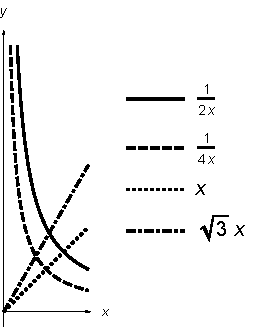
\includegraphics[]{figures/cjf1.pdf}
%     \caption{}
%     \label{cjfs}
% \end{figure}

% \begin{figure}[H]
%     \centering
%     \subfigure[]{
%         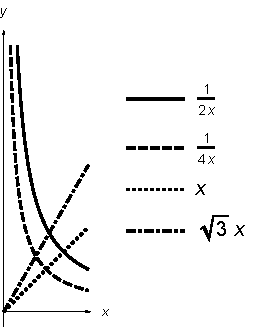
\includegraphics[]{figures/cjf1.pdf}
%     }
%     \subfigure[]{
%         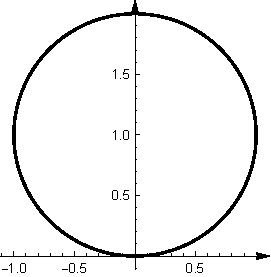
\includegraphics[]{figures/cjf2.pdf}
%     }
%     \caption{}
%     \label{cjfs}
% \end{figure}

\begin{example}
    设函数 $f(u)$ 连续,区域 $D=\qty{(x,y)\mid x^2+y^2\leqslant 2y}$,则 $\displaystyle\iint\limits_D f(xy)\dd x\dd y$.
    \begin{tasks}(2)
        \task $\displaystyle \int_{-1}^{1}\dd x\int_{-\sqrt{1-x^2}}^{\sqrt{1-x^2}}f(xy)\dd y.$
        \task $\displaystyle 2\int_{0}^{2}\dd y\int_{0}^{\sqrt{2y-y^2}}f(xy)\dd x.$
        \task $\displaystyle \int_{0}^{\pi}\dd \theta\int_{0}^{2\sin\theta}f\qty(r^2\sin\theta\cos\theta)\dd r.$
        \task $\displaystyle \int_{0}^{\pi}\dd \theta\int_{0}^{2\sin\theta}f\qty(r^2\sin\theta\cos\theta)r\dd r.$
    \end{tasks}
\end{example}
\begin{solution}
    在直角坐标系下
    $$\iint\limits_Df(xy)\dd x\dd y=\int_{0}^{2}\dd y\int_{-\sqrt{1-(y-1)^2}}^{\sqrt{1-(y-1)^2}}f(xy)\dd x=\int_{-1}^{1}\dd x\int_{1-\sqrt{1-x^2}}^{1+\sqrt{1-x^2}}f(xy)\dd y$$
    故排除 A、B,在极坐标下
    $$\iint\limits_D f(xy)\dd x\dd y=\int_{0}^{\pi}\dd \theta\int_{0}^{2\sin\theta}f\qty(r^2\sin\theta\cos\theta)r\dd r$$
    故选 D.
\end{solution}

% \begin{example}
%     计算下列积分:
%     \setcounter{magicrownumbers}{0}
%     \begin{table}[H]
%         \centering
%         \begin{tabular}{l | l}
%             (\rownumber{}) (2016 数一) $\displaystyle\iint\limits_{\substack{2\leqslant r\leqslant 2(1+\cos\theta)\\-\frac{\pi}{2}\leqslant \theta\leqslant \frac{\pi}{2}}}x\dd x\dd y$. & (\rownumber{}) 
%         \end{tabular}
%     \end{table}
% \end{example}

\begin{example}
    计算三重积分 $\displaystyle I=\iiint\limits_\Omega z\dd x\dd y\dd z$,其中 $\Omega$ 是两个球面 $x^2+y^2+z^2=2z$ 和 $x^2+y^2+z^2=z$ 围成的区域.
\end{example}
\begin{solution}
    由球坐标变化,$\begin{cases}
            x=r\sin\varphi \cos\theta \\
            y=r\sin\varphi \sin\theta \\
            z=r\cos\varphi
        \end{cases}$,则 $\Omega'=\qty{0\leqslant \theta\leqslant 2\pi,0\leqslant\varphi\leqslant\dfrac{\pi}{2},\cos\varphi\leqslant r\leqslant 2\cos\varphi}$,则
    \begin{flalign*}
        I & =\int_{0}^{2\pi}\dd \theta\int_{0}^{\frac{\pi}{2}}\dd \varphi\int_{\cos\varphi}^{2\cos\varphi}r\cos\varphi\cdot r^2\sin\varphi\dd r=2\pi\int_{0}^{\frac{\pi}{2}}\sin\varphi\cos\varphi\dd \varphi\int_{\cos\varphi}^{2\cos\varphi}r^3\dd r \\
          & =\dfrac{15\pi2}{2}\int_{0}^{\frac{\pi}{2}}\sin\varphi\cos^5\varphi\dd \varphi=\dfrac{5\pi}{4}.
    \end{flalign*}
\end{solution}

\begin{example}
    设积分区域 $\Omega_t:x^2+y^2+z^2\leqslant 2tz,~f(0)=0,~f'(0)=15$,求极限 $$\lim_{t\to0^+}\dfrac{1}{t^5}\iiint\limits_{\Omega_t}f\qty(x^2+y^2+z^2)\dd V.$$
\end{example}
\begin{solution}
    \textbf{法一: }由三重积分的球坐标计算方法,积分区域可用球坐标变量表示为
    $$0\leqslant \theta\leqslant 2\pi ,~0\leqslant \varphi\leqslant \dfrac{\pi}{2},~0\leqslant r\leqslant 2t\cos\varphi$$
    故三重积分表示为 $\displaystyle g(t)=\int_{0}^{2\pi}\dd \theta\int_{0}^{\frac{\pi}{2}}\sin\varphi\dd \varphi\int_{0}^{2t\cos\varphi}f\qty(r^2)r^2\dd r$,设 $F'(r)=f\qty(r^2)r^2$,则
    \begin{flalign*}
        g(t) & =2\pi\int_{0}^{\frac{\pi}{2}}\qty[F(2t\cos\varphi)-F(0)]\sin\varphi\dd \varphi=2\pi\int_{0}^{\frac{\pi}{2}}F(2t\cos\varphi)\sin\varphi\dd \varphi-2\pi F(0)\int_{0}^{\frac{\pi}{2}}\sin\varphi\dd \varphi \\
             & =-2\pi\int_{0}^{\frac{\pi}{2}}F(2t\cos\varphi)\dd \cos\varphi-2\pi F(0)=\dfrac{\pi}{t}\int_{0}^{2t}F(u)\dd u-2\pi F(0)
    \end{flalign*}
    故
    \begin{flalign*}
        I & =\lim_{t\to0^+}\dfrac{1}{t^5}\iiint\limits_{\Omega_t}f\qty(x^2+y^2+z^2)\dd V=\pi\lim_{t\to0^+}\dfrac{\displaystyle\int_{0}^{2t}F(u)\dd u-2tF(0)}{t^6}\xlongequal[]{L'}\pi\lim_{t\to0^+}\dfrac{2F(2t)-2F(0)}{6t^5} \\
          & =\dfrac{\pi}{3}\lim_{t\to0^+}\dfrac{F(2t)-F(0)}{t^5}\xlongequal[]{L'}\dfrac{\pi}{3}\lim_{t\to0^+}\dfrac{2F'(2t)}{5t^4}=\dfrac{2\pi}{15}\lim_{t\to0^+}\dfrac{4t^2f\qty(4t^2)}{t^4}=\dfrac{32\pi}{15}f'(0)=32\pi.
    \end{flalign*}
    \textbf{法二: }有题意可假设 $f(x)=15x+o(x)$,并令 $\displaystyle g(t)=\iiint\limits_{\Omega_t}f\qty(x^2+y^2+z^2)\dd V$,于是
    \begin{flalign*}
        g(t) & =\iiint\limits_{\Omega_t}\qty[15\qty(x^2+y^2+z^2)+o\qty(x^2+y^2+z^2)]\dd V =\int_{0}^{2\pi}\dd \theta\int_{0}^{\frac{\pi}{2}}\dd \varphi\int_{0}^{2t\cos\varphi}\qty[15r^2+o\qty(r^2)]r^2\sin\varphi\dd r \\
             & =2\pi\int_{0}^{\frac{\pi}{2}}\sin\varphi\qty[3r^5+o\qty(r^5)]\biggl |_{0}^{2t\cos\varphi}\dd \varphi=-6\pi\cdot32t^5\int_{0}^{\frac{\pi}{2}}\cos^5\varphi\dd \cos\varphi+o\qty(t^5)=32\pi t^5+o\qty(t^5)
    \end{flalign*}所以 $\displaystyle\lim_{t\to0^+}\dfrac{g(t)}{t^5}=32\pi.$
\end{solution}

\begin{example}
    设 $f(x)$ 是 $(0,+\infty)$ 上连续可导的函数,$f(x)\neq0$ 且 $\displaystyle\lim_{x\to+\infty}\dfrac{xf'(x)}{f(x)}=c>0$,记
    $$F(t)=\iiint\limits_{x^2+y^2+z^2\leqslant t^2}f\qty(\sqrt{x^2+y^2+z^2})\dd V,~~G(t)=\iint\limits_{x^2+y^2\leqslant t^2}f\qty(\sqrt{x^2+y^2})\dd \sigma$$
    求函数 $h(t)$,使得 $\displaystyle\lim_{t\to+\infty}\dfrac{F(t)}{h(t)G(t)}=1.$
\end{example}
\begin{solution}
    由三重积分的球坐标计算公式和二重积分的极坐标计算公式,得
    \begin{flalign*}
        F(t) & =\int_{0}^{2\pi}\dd \theta\int_{0}^{\pi}\sin\varphi\dd \varphi\int_{0}^{t}f(r)r^2\dd r=4\pi\int_{0}^{t}f(r)r^2\dd r \\
        G(t) & =\int_{0}^{2\pi}\dd \theta\int_{0}^{t}f(r)r\dd r=2\pi\int_{0}^{t}f(r)r^2\dd r
    \end{flalign*}
    由 $\displaystyle\lim_{x\to+\infty}\dfrac{xf'(x)}{f(x)}=c>0$ 知,$\exists X_0>0$,当 $x>X_0$ 时,$f(x)$ 与 $f'(x)$ 同号,故 $f(x)>0$ 时,$f(x)$ 单调递增,则
    $$\lim_{t\to+\infty}F(t)=+\infty,~~\lim_{t\to+\infty}G(t)=+\infty,~~\int_{X_0}^{+\infty}f(t)\dd t=+\infty$$
    那么
    \begin{flalign*}
        \lim_{t\to+\infty}\dfrac{F(t)}{tG(t)} & =\lim_{t\to+\infty}\dfrac{\displaystyle 4\pi\int_{0}^{t}f(r)r^2\dd r}{\displaystyle 2\pi t\int_{0}^{t}f(t)t\dd t}=2\lim_{t\to+\infty}\dfrac{\displaystyle\int_{0}^{t}f(r)r^2\dd r}{\displaystyle t\int_{0}^{t}f(t)t\dd t}\xlongequal{L'}2\lim_{t\to+\infty}\dfrac{f(t)t^2}{\displaystyle\int_{0}^{t}f(t)t\dd t+f(t)t^2} \\
                                              & \xlongequal{L'}2\lim_{t\to+\infty}\dfrac{2tf(t)+t^2f'(t)}{3tf(t)+t^2f'(t)}=2\lim_{t\to+\infty}\dfrac{2\dfrac{tf'(t)}{f(t)}}{3+\dfrac{tf'(t)}{f(t)}}=\dfrac{2(2+c)}{3+c}
    \end{flalign*}
    故 $\displaystyle \lim_{t\to+\infty}\dfrac{F(t)}{\dfrac{2(2+c)}{3+c}tG(t)}=1$,所以取 $h(t)=\dfrac{2(2+c)}{3+c}t$ 即为所求函数.
\end{solution}

\subsubsection{Jacobian 行列式}

\begin{example}
    设 $D$ 是 $y=\sqrt{x},~x=\sqrt{y}$ 和 $x^2+y^2-x-y+\dfrac{1}{4}=0,~\qty(x,y\in\qty[0,\dfrac{1}{2}])$ 围成的封闭区域,求积分
    $$\iint\limits_D\qty(x-y^2)\qty(y-x^2)(1-4xy)\dd x\dd y.$$
\end{example}
\begin{solution}
    令 $u=x-y^2,~v=y-x^2$,那么 $D'=\qty{(u,v)|u,v\geqslant 0,u+v\leqslant\dfrac{1}{4}}$
    $$|J|=\qty|\pdv{(x,y)}{(u,v)}|=\dfrac{1}{\qty|\displaystyle\pdv{(u,v)}{(x,y)}|}=\dfrac{1}{|1-4xy|}$$
    \begin{flalign*}
        \text{原式}=\iint\limits_{D'}uv\dd u\dd v=\int_{0}^{\frac{1}{4}}\dd u\int_{0}^{\frac{1}{4}-u}uv\dd v=\int_{0}^{\frac{1}{4}}\qty(\dfrac{1}{2}u^3-\dfrac{1}{4}u^2+\dfrac{1}{32}u)\dd u=\dfrac{1}{6144}.
    \end{flalign*}
\end{solution}

\begin{example}
    设 $z=z(x,y)$ 是由 $\varphi(y-bz)=x-az$ 确定的隐函数,其中 $\varphi$ 是连续可微函数,且 $a-b\varphi'(y-bz)\neq 0$,求二重积分
    $$I=\iiint\limits_D\qty(az'_x+bz_y')\e^{\frac{x-y}{x+y}}\dd x\dd y$$
    其中 $D$ 是由 $x=0,~y=0,~x+y=1$ 所围成的区域.
\end{example}
\begin{solution}
    令 $F(x,y,z)=x-az-\varphi(y-bz)$,那么 $$F_x'=1,~F_y'=-\varphi'(y-bz),~F_z'=-a+b\varphi'(y-bz)$$
    当 $a-b\varphi'(y-bz)=\neq 0$ 时,由隐函数求导公式,得
    $$z_x'=-\dfrac{F_x'}{F_z'}=\dfrac{1}{a-b\varphi'(y-bz)},~z_y'=-\dfrac{F_y'}{F_z'}=-\dfrac{\varphi'(y-bz)}{a-b\varphi'(y-bz)}$$
    于是 $az_x'+bz_y'=1$,代入被积函数表达式,得 $\displaystyle I=\displaystyle\iint\limits_D \e^{\frac{x-y}{x+y}}\dd x\dd y$
    令 $u=x-y,~v=x+y,~J=\dfrac{\partial(x,y)}{\partial(u,v)}=\dfrac{1}{2}$,且变换后的积分区域为 $D_{uv}=\qty{(u,v):-v\leqslant u\leqslant v,0\leqslant v\leqslant 1}$,所以二重积分化为
    \begin{flalign*}
        I=\iint\limits_{D_{uv}}\e^{\frac{u}{v}}\dfrac{1}{2}\dd u\dd v=\dfrac{1}{2}\int_{0}^{1}\dd v\int_{-v}^{v}\e^{\frac{u}{v}}\dd u=\dfrac{\e-\e^{-1}}{4}.
    \end{flalign*}
\end{solution}

\begin{example}[2007 湖南大学]
    计算积分 $$I=\iint\limits_D\dfrac{(x+y)\qty[\ln(x+y)-\ln y]}{\sqrt{2-x-y}}\dd x\dd y$$
    其中区域 $D$ 为 $x=0,x+y=1,y=x$ 所围成的三角形区域.
\end{example}
\begin{solution}
    原式改写为 $\displaystyle I=\iint\limits_D\dfrac{(x+y)\ln\qty(1+\dfrac{x}{y})}{\sqrt{2-(x+y)}}\dd x\dd y$,则令 $u=x+y,v=\dfrac{x}{y}$,那么 $\begin{cases}
            x=\dfrac{uv}{1+v} \\[6pt]
            y=\dfrac{u}{1+v}
        \end{cases}$,并且
    $$J=\pdv{(x,y)}{(u,v)}=\begin{vmatrix}
            \dfrac{v}{1+v} & \dfrac{u}{(1+v)^2}  \\[6pt]
            \dfrac{1}{1+v} & \dfrac{-u}{(1+v)^2}
        \end{vmatrix}=-\dfrac{u}{(1+v)^2} $$
    \begin{flalign*}
        \text{原式} & =\iint\limits_{D_{uv}}\dfrac{u\ln(1+v)}{\sqrt{2-u}}|J|\dd u\dd v=\iint\limits_{D_{uv}}\dfrac{u\ln(1+v)}{\sqrt{2-u}}\cdot\dfrac{u}{(1+v)^2}\dd u\dd v                                   \\
                    & =\int_{0}^{1}\dfrac{u^2}{\sqrt{2-u}}\dd u\cdot\int_{0}^{1}\dfrac{\ln(1+v)}{(1+v)^2}\dd v=\dfrac{2}{15}\qty(32\sqrt{2}-43)\cdot\dfrac{1}{2}(1-\ln 2)=\dfrac{32\sqrt{2}-43}{15}(1-\ln2).
    \end{flalign*}
\end{solution}

% \begin{example}
%     计算积分 $I=\displaystyle\iint\limits_D \dfrac{3x}{y^2+xy^3}\dd x\dd y$,其中 $D$ 为平面曲线 $xy=1,xy=3,y^2=x,y^2=3x$ 所围成的有界闭区域.
% \end{example}
% \begin{solution}
% 
% \end{solution}

\begin{example}
    设 $\Omega$ 是由曲面 $z=y^2,z=4y^2~~(y>0)$,平面 $z=x,z=2x$ 及 $z=2$ 所围区域,
    求积分 $$\iiint\limits_\Omega \frac{z\sqrt{z}}{y^3}\cos\frac{z}{y^2}\dd x\dd y\dd z.$$
\end{example}
\begin{solution}
    令 $\displaystyle u=\frac{z}{y^2},v=\frac{z}{x},z=z$,即 $\displaystyle x=\frac{z}{v},y=\sqrt{\frac{z}{u}},z=z$,$\Omega':~0\leqslant z\leqslant 2,1\leqslant v\leqslant 2,1\leqslant u\leqslant 4$.
    $$J=\frac{\partial (x,y,z)}{\partial (u,v,z)}=\begin{vmatrix}
            0                                             & \displaystyle-\frac{z}{v^2} & \displaystyle\frac{1}{v}                    \\[6pt]
            \displaystyle-\frac{1}{2}\sqrt{\frac{z}{u^3}} & 0                           & \displaystyle\frac{1}{2}\sqrt{\frac{1}{uz}} \\[6pt]
            0                                             & 0                           & 1
        \end{vmatrix}=-\frac{z}{2v^2}\left(\frac{z}{u}\right)^{\frac{3}{2}}$$
    \begin{flalign*}
        \iiint\limits_\Omega\frac{z\sqrt{z}}{y^3}\cos\frac{z}{y^2}\dd x\dd y\dd z & =\iiint\limits_{\Omega'}u^{\frac{3}{2}}\cos u |J|\dd u\dd v\dd z
        =\iiint\limits_{\Omega'}u^{\frac{3}{2}}\cos u\cdot\frac{z}{2v^2}\left(\frac{z}{u}\right)^{\frac{3}{2}}\dd u\dd v\dd z                                                                                 \\
                                                                                  & =\frac{1}{2}\int_1^4\cos u\dd u\int_1^2\frac{1}{v^2}\dd v\int_0^2z^{\frac{5}{2}}\dd z=\frac{4\sqrt{2}}{7}(\sin 4-\sin 1).
    \end{flalign*}
\end{solution}

\begin{example}
    设 $x=x(u,v),~y=y(u,v)$ 有连续偏导数,一一对应地将区域 $D'$ 映射到 $xOy$ 平面的区域 $D$,满足 $J\neq0$,且
    $$\pdv{x}{u}=\pdv{y}{v},~\pdv{x}{v}=-\pdv{y}{u}$$
    证明: $\displaystyle \iint\limits_D\qty[\qty(\pdv{f}{x})^2+\qty(\pdv{f}{y})^2]\dd x\dd y=\iint\limits_{D'}\qty[\qty(\pdv{f}{u})^2+\qty(\pdv{f}{v})^2]\dd u\dd v$.
\end{example}
\begin{proof}[{\songti \textbf{证}}]
    由已知得 $$\qty(\pdv{f}{u})^2=\qty(\pdv{f}{x}\cdot\pdv{x}{u}+\pdv{f}{y}\cdot\pdv{y}{u})^2=\qty(\pdv{f}{x}\cdot\pdv{y}{v}+\pdv{f}{y}\cdot\pdv{y}{u})^2$$
    $$\qty(\pdv{f}{v})^2=\qty(\pdv{f}{x}\cdot\pdv{x}{v}+\pdv{f}{y}\cdot\pdv{y}{v})^2=\qty(-\pdv{f}{x}\cdot\pdv{y}{u}+\pdv{f}{y}\cdot\pdv{y}{v})^2$$
    两式相加
    \begin{flalign*}
        \qty(\pdv{f}{u})^2+\qty(\pdv{f}{v})^2 & =\qty(\pdv{f}{x})^2\qty[\qty(\pdv{y}{v})^2+\qty(\pdv{y}{u})^2]+\qty(\pdv{f}{y})^2\qty[\qty(\pdv{y}{u})^2+\qty(\pdv{y}{v})^2] \\
                                              & =\qty[\qty(\pdv{f}{x})^2+\qty(\pdv{f}{y})^2]\qty[\qty(\pdv{y}{u})^2+\qty(\pdv{y}{v})^2]
    \end{flalign*}
    另外 $$J=\pdv{(x,y)}{(u,v)}=\begin{vmatrix}
            \displaystyle\pdv{x}{u} & \displaystyle\pdv{x}{v} \\[6pt]
            \displaystyle\pdv{y}{u} & \displaystyle\pdv{y}{v}
        \end{vmatrix}=\pdv{x}{u}\cdot\pdv{y}{v}-\pdv{x}{v}\cdot\pdv{y}{u}=\qty(\pdv{y}{u})^2+\qty(\pdv{y}{v})^2$$
    从而 $$\dd u\dd v=\qty|J^{-1}|\dd x\dd y=\dfrac{\dd x\dd y}{\qty(\displaystyle\pdv{y}{u})^2+\qty(\displaystyle\pdv{y}{v})^2}$$
    综上所述,得证 $\displaystyle \iint\limits_D\qty[\qty(\pdv{f}{x})^2+\qty(\pdv{f}{y})^2]\dd x\dd y=\iint\limits_{D'}\qty[\qty(\pdv{f}{u})^2+\qty(\pdv{f}{v})^2]\dd u\dd v$.
\end{proof}

\subsubsection{四重积分换元}

\begin{example}\scriptsize\linespread{0.8}
    求 $\displaystyle\iiiint\limits_V\sqrt{\dfrac{1-x^2-y^2-z^2-u^2}{1+x^2+y^2+z^2+u^2}}\dd x\dd y\dd z\dd u$,其中 $V$ 为 $x,y,z,u\geqslant 0$,$x^2+y^2+z^2+u^2\leqslant 1$.
\end{example}
\begin{solution}\scriptsize\linespread{0.8}
    \textbf{法一: }用球坐标 $$x=r\cos\psi,~y=r\sin\psi\cos\varphi,~z=r\sin\psi\sin\varphi\cos\theta,~u=r\sin\psi\sin\varphi\sin\theta$$
    此时 $$J=\pdv{(x,y,z,u)}{(r,\psi,\varphi,\theta)}=r^3\sin^2\phi\sin\varphi,~x^2+y^2+z^2+u^2=r^2$$
    $$V=\qty{(r,\phi,\varphi,\theta)\biggl | 0\leqslant \phi\leqslant \dfrac{\pi}{2},~0\leqslant \varphi\leqslant \dfrac{\pi}{2},~0\leqslant \theta\leqslant \dfrac{\pi}{2},~0\leqslant r\leqslant 1}$$
    故原积分
    \begin{flalign*}
        I & =\int_{0}^{\frac{\pi}{2}}\dd\theta\int_{0}^{\frac{\pi}{2}}\sin\varphi\dd \varphi\int_{0}^{\frac{\pi}{2}}\sin^2\psi\dd\psi\int_{0}^{1}\sqrt{\dfrac{1-r^2}{1+r^2}}r^3\dd r=\dfrac{\pi^2}{16}\int_{0}^{1}\sqrt{\dfrac{1-r^2}{1+r^2}}r^2\dd r^2 \\
          & \xlongequal[]{r^2=\sin t}\dfrac{\pi^2}{16}\int_{0}^{\frac{\pi}{2}}\qty(\sin t-\sin^2t)\dd t=\dfrac{\pi^2}{16}\qty(1-\dfrac{\pi}{4}).
    \end{flalign*}
    \textbf{法二: }用双极坐标 $$x=r\cos\theta,~y=r\sin\theta,~z=\rho\cos\varphi,~u=\rho\sin\varphi$$
    此时 $$J=\pdv{(x,y,z,u)}{(r,\theta,\rho,\varphi)}=r\rho,~x^2+y^2+z^2+u^2=r^2+\rho^2$$
    $$V=\qty{(r,\theta,\rho,\varphi)\biggl |0\leqslant \theta\leqslant \dfrac{\pi}{2},0\leqslant \varphi\leqslant\dfrac{\pi}{2},r\geqslant0,\rho\geqslant 0,r^2+\rho^2\leqslant 1}$$
    故原积分
    \begin{flalign*}
        I=\iiiint\limits_V\sqrt{\dfrac{1-r^2-\rho^2}{1+r^2+\rho^2}}r\rho\dd r\dd \rho\dd\theta\dd \varphi=\int_{0}^{\frac{\pi}{2}}\dd\theta\int_{0}^{\frac{\pi}{2}}\dd\varphi\iint\limits_{\substack{r^2+\rho^2\leqslant 1 \\ r,\rho\geqslant0}}\sqrt{\dfrac{1-r^2-\rho^2}{1+r^2+\rho^2}}r\rho\dd r\dd \rho=\dfrac{\pi^2}{16}\qty(1-\dfrac{\pi}{4}).
    \end{flalign*}
\end{solution}

\subsubsection{分区积分及对称性的应用}

\begin{theorem}[重积分的对称性]
    \begin{enumerate}[label=(\arabic{*})]
        \item 二重积分情形:
              \begin{enumerate}[label=(\roman{*})]
                  \item 若积分区域 $ D $ 关于 $ x $ 轴对称,而 $ D_{1}$ 是 $ D $ 中对应于 $ y \geqslant 0 $ 的部分,则
                        $$\iint\limits_{D} f(x, y) \dd  x \dd  y=\begin{cases}
                                2 \displaystyle\iint_{D_{1}} f(x, y) \dd  x \dd  y, & f(x,-y)=f(x, y),   \\
                                0,                                                  & f(x,-y)=-f(x, y) .
                            \end{cases}$$
                  \item 若积分区域 $ D $ 关于 $ y $ 轴对称,而 $ D_{1} $ 是 $ D $ 中对应于 $ x \geqslant 0 $ 的部分,则
                        $$\iint\limits_{D} f(x, y) \dd  x \dd  y=\begin{cases}
                                2 \displaystyle\iint_{D_{1}} f(x, y) \dd  x \dd  y, & f(-x, y)=f(x, y),   \\
                                0,                                                  & f(-x, y)=-f(x, y) .
                            \end{cases}$$
                  \item 若积分区域 $ D $ 关于 $ x $ 轴和 $ y $ 轴均对称,而 $ D_{1} $ 是 $ D $ 中对应于 $ x \geqslant 0, y \geqslant 0 $ 的部分,则
                        $$\iint\limits_{D} f(x, y) \dd  x \dd  y=\begin{cases}
                                4 \displaystyle\iint_{D_{1}} f(x, y) \dd  x \dd  y, & f(-x, y)=f(x,-y)=f(x, y),                \\
                                0,                                                  & f(-x, y) \text { 或 } f(x,-y)=-f(x, y) .
                            \end{cases}$$
              \end{enumerate}
        \item 三重积分情形:
              \begin{enumerate}[label=(\roman{*})]
                  \item 若积分区域 $ \Omega $ 关于 $ x O y $ 平面对称,而 $ \Omega_{1} $ 是 $ \Omega $ 中对应于 $ z \geqslant 0 $ 的部分,则
                        $$\iiint\limits_{\Omega} f(x, y, z) \dd  v=\begin{cases}
                                2 \displaystyle\iiint\limits_{\Omega_{1}} f(x, y, z) \dd  v, & f \text { 关于 } z \text { 为偶函数, } \\
                                0,                                                           & f \text { 关于 } z \text { 为奇函数. }
                            \end{cases}$$
                        如果积分区域 $ \Omega $ 关于 $ x O z $ 或 $ y O z $ 平面对称,那么也有类似的结果.
                  \item 若积分区域 $ \Omega $ 关于 $ x O y $ 平面和 $ x O z $ 平面均对称,而 $ \Omega_{1} $ 是 $ \Omega $ 中对应于 $ z \geqslant 0 ,  y \geqslant 0 $ 的部分,则
                        $$\iiint\limits_{\Omega} f(x, y, z) \dd  v=\begin{cases}
                                4 \displaystyle\iiint\limits_{\Omega_{1}} f(x, y, z) \dd  v, & f \text { 关于 } y, z \text { 均为偶函数, }           \\
                                0,                                                           & f \text { 关于 } y \text { 或 } z \text { 为奇函数. }
                            \end{cases}$$
                        如果积分区域 $ \Omega $ 关于 $ x O z $ 平面和 $ y O z $ 平面均对称,或者关于 $ x O y $ 平面和 $ y O z $ 平面均对称,那么也有类似的结果.
                  \item 如果积分区域 $ \Omega $ 关于 $3$ 个坐标平面均对称,而 $ \Omega_{1} $ 是 $ \Omega $ 中位于第一卦限的部分,则
                        $$\iiint\limits_{\Omega} f(x, y, z) \dd  v=\begin{cases}
                                8 \displaystyle\iiint\limits_{\Omega_{1}} f(x, y, z) \dd  v, & f \text { 关于 } x, y, z \text { 均为偶函数, }                       \\
                                0,                                                           & f \text { 关于 } x \text { 或 } y \text { 或 } z \text { 为奇函数. }
                            \end{cases}$$
              \end{enumerate}
    \end{enumerate}
    \index{重积分的对称性}
\end{theorem}

\begin{example}
    计算积分.
    \setcounter{magicrownumbers}{0}
    \begin{table}[H]
        \centering
        \begin{tabular}{l | l}
            (\rownumber{}) $\displaystyle \iint\limits_{[0,1]\times [0,1]}\qty|xy-\dfrac{1}{4}|\dd x\dd y$.                                                       & (\rownumber{}) $\displaystyle\iint\limits_{x^2+y^2\leqslant 5}\mathrm{sgn}\qty(x^2-y^2+3)\dd x\dd y$.                           \\
            (\rownumber{}) $\displaystyle\iint\limits_{|x|\leqslant 1,0\leqslant y\leqslant 2}\sqrt{\qty|y-x^2|}\dd x\dd y$.                                      & (\rownumber{}) $\displaystyle \iint\limits_{0\leqslant x,y\leqslant 2}[x+y]\dd x\dd y$ ($[\cdot]$ 表示不大于 $\cdot$ 最大整数). \\
            (\rownumber{}) $\displaystyle\iint\limits_{x^2+y^2\leqslant a^2}\dfrac{|xy|\qty(1+\mathrm{e}^{x^2})}{2+\mathrm{e}^{x^2}+\mathrm{e}^{y^2}}\dd x\dd y.$ & (\rownumber{}) (2024 数一) $\displaystyle\iint\limits_{\substack{\sqrt{1-y^2}\leqslant x\leqslant 1                             \\-1\leqslant y\leqslant 1}}\dfrac{x}{\sqrt{x^2+y^2}}\dd x\dd y.$
        \end{tabular}
    \end{table}
\end{example}
\begin{solution}
    \begin{enumerate}[label=(\arabic{*})]
        \item $\qty|xy-\dfrac{1}{4}|=\begin{cases}
                      \dfrac{1}{4}-xy , & (x,y)\text{ 在双曲线 }xy=\dfrac{1}{4}\text{ 之下} \\[6pt]
                      xy-\dfrac{1}{4} , & (x,y)\text{ 在双曲线 }xy=\dfrac{1}{4}\text{ 之上}
                  \end{cases}$,如图 (a) 所示,将积分区域划分为三个区域,于是
              \begin{flalign*}
                  I & =\iint\limits_{D_2\cup D_3}\qty(\dfrac{1}{4}-xy)\dd x\dd y+\iint\limits_{D_1}\qty(xy-\dfrac{1}{4})\dd x\dd y                                                                                                                 \\
                    & =\int_{0}^{\frac{1}{4}}\dd x\int_{0}^{1}\qty(\dfrac{1}{4}-xy)\dd y+\int_{\frac{1}{4}}^{1}\dd x\int_{0}^{\frac{1}{4x}}\qty(\dfrac{1}{4}-xy)\dd y+\int_{\frac{1}{4}}^{1}\dd x\int_{\frac{1}{4x}}^{1}\qty(xy-\dfrac{1}{4})\dd y \\
                    & =\dfrac{3}{64}+\dfrac{\ln 2}{16}+\dfrac{1}{16}\qty(\dfrac{3}{4}+\ln 2)=\dfrac{1}{8}\qty(\dfrac{3}{4}+\ln 2).
              \end{flalign*}
        \item 被积函数 $\mathrm{sgn}\qty(x^2-y^2+3) =\begin{cases}
                      1  , & x^2-y^2+3>0 \\
                      0  , & x^2-y^2+3=0 \\
                      -1 , & x^2-y^2+3<0
                  \end{cases}$,
              如图 (b) 所示,被积函数和积分区域都关于坐标轴对称,因此只要计算第一象限的部分,再乘 $4$ 即为原积分值,故
              \begin{flalign*}
                  \text{原式} & =4\iint\limits_{\substack{x^2+y^2\leqslant5                                                                                                    \\x,y\geqslant 0}}\mathrm{sgn}\qty(x^2-y^2+3)\dd x\dd y=4\int_{0}^{1}\dd x\int_{0}^{\sqrt{x^2+3}}\dd y-4\int_{0}^{1}\dd x\int_{\sqrt{x^2+5}}^{\sqrt{5-x^2}}\dd y+4\int_{1}^{\sqrt{5}}\dd x\int_{0}^{\sqrt{5-x^2}}\dd y \\
                              & =8\int_{0}^{1}\sqrt{x^2+3}\dd x-4\int_{0}^{1}\sqrt{5-x^2}\dd x+4\int_{0}^{\sqrt{5}}\sqrt{5-x^2}\dd x=6\ln 3+5\pi-20\arcsin\dfrac{1}{\sqrt{5}}.
              \end{flalign*}
        \item 如图 (c) 所示,
              \begin{flalign*}
                  I & =\iint\limits_{|x|\leqslant 1,0\leqslant y\leqslant 2}\sqrt{\qty|y-x^2|}\dd x\dd y=\iint\limits_{|x|\leqslant 1,x^2\leqslant y\leqslant 2}\sqrt{y-x^2}\dd x\dd y+\iint\limits_{|x|\leqslant 1,0\leqslant y\leqslant x^2}\sqrt{x^2-y}\dd x\dd y \\
                    & =\int_{-1}^{1}\dd x\int_{x^2}^{2}\sqrt{y-x^2}\dd y+\int_{-1}^{1}\dd x\int_{0}^{x^2}\sqrt{x^2-y}\dd y=\dfrac{\pi}{2}+\dfrac{5}{3}.
              \end{flalign*}
        \item 如图 (d) 所示,$\displaystyle\text{原式}=S_{ABCD}+2S_{CDEF}+3S_{\triangle EFG}+3S_{\triangle CDG}=6.$
        \item 积分区域关于 $x,y$ 都对称,且具有轮换对称性,则有
              \begin{flalign*}
                  \text{原式} & =4\iint\limits_{\substack{x^2+y^2\leqslant a^2 \\ x,y\geqslant0}}\dfrac{xy\qty(1+\mathrm{e}^{x^2})}{2+\mathrm{e}^{x^2}+\mathrm{e}^{y^2}}\dd x\dd y=2\iint\limits_{\substack{x^2+y^2\leqslant a^2\\ x,y\geqslant0}}\qty[\dfrac{xy\qty(1+\mathrm{e}^{x^2})}{2+\mathrm{e}^{x^2}+\mathrm{e}^{y^2}}+\dfrac{yx\qty(1+\mathrm{e}^{y^2})}{2+\mathrm{e}^{y^2}+\mathrm{e}^{x^2}}]\dd x\dd y\\
                              & =2\iint\limits_{\substack{x^2+y^2\leqslant a^2 \\ x,y\geqslant0}}xy\dd x\dd y=2\int_{0}^{\frac{\pi}{2}}\cos \theta\sin\theta\dd \theta\int_{0}^{a}\rho^3\dd \rho=\dfrac{a^4}{4}.
              \end{flalign*}
        \item 积分区域关于 $x$ 轴对称,被积函数是 $y$ 的偶函数,那么
              \begin{flalign*}
                  \text{原式} & =2\iint\limits_{\substack{\sqrt{1-y^2}\leqslant x\leqslant 1                                                             \\0\leqslant y\leqslant 1}}\dfrac{x}{\sqrt{x^2+y^2}}\dd x\dd y=2\int_{0}^{1}\dd y\int_{\sqrt{1-y^2}}^{1}\dfrac{x}{\sqrt{x^2+y^2}}\dd x=2\int_{0}^{1}\dd y\int_{\sqrt{1-y^2}}^{1}\dfrac{\dd \qty(x^2+y^2)}{\sqrt{x^2+y^2}}\\
                              & =2\int_{0}^{1}\sqrt{1+y^2}\dd y-2=\eval{y\sqrt{1+y^2}+\ln\qty(y+\sqrt{1+y^2})}_{0}^{1}-2=\sqrt{2}-2+\ln\qty(1+\sqrt{2}).
              \end{flalign*}
    \end{enumerate}
    \begin{figure}[H]
        \centering
        \subfigure[]{
            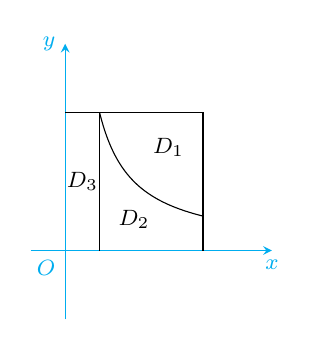
\begin{tikzpicture}[->,samples=100,>=stealth,domain=0.25:1,scale=1.75,font=\footnotesize]
                \coordinate (xMin) at (-0.25,0);
                \coordinate (xMax) at (1.5,0);
                \coordinate (yMin) at (0,-0.5);
                \coordinate (yMax) at (0,1.5);
                % \filldraw[fill=magenta!30] (0,0)--(0.25,0)--(0.25,1)--(0,1)--cycle;
                \draw[->,cyan] (xMin)--(0,0) node [below left] {$O$}--(xMax) node[below] {$x$};
                \draw[->,cyan] (yMin)--(yMax) node [left] {$y$};
                \draw[-] plot(\x,{1/(4*\x)});
                \draw[-] (1,0)--(1,1)--(0,1);
                \draw[-] (0.25,0)--(0.25,1);
                \node at(0.125,0.5) {$D_3$};
                \node at(0.5,0.225) {$D_2$};
                \node at(0.75,0.75) {$D_1$};
            \end{tikzpicture}
        }
        \subfigure[]{
            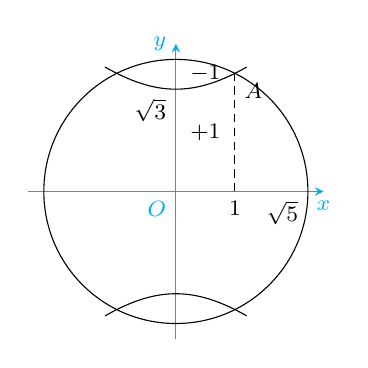
\begin{tikzpicture}[->,samples=100,>=stealth,domain=-1.2:1.2,scale=0.75,font=\footnotesize]
                \coordinate (xMin) at (-2.5,0);
                \coordinate (xMax) at (2.5,0);
                \coordinate (yMin) at (0,-2.5);
                \coordinate (yMax) at (0,2.5);
                \draw[->,cyan] (xMin)--(0,0) node [below left] {$O$}--(xMax) node[below] {$x$};
                \draw[->,cyan] (yMin)--(yMax) node [left] {$y$};
                \draw[-] (0,0) circle ({sqrt(5)});
                \draw[-] plot(\x,{sqrt(\x*\x+3)});
                \draw[-] plot(\x,{-sqrt(\x*\x+3)});
                \node at (1,2) [below right] {$A$};
                \node at (1,0) [below] {$1$};
                \node at ({sqrt(5)},0) [below left] {$\sqrt{5}$};
                \draw[densely dashed,-] (1,0)--(1,2);
                \node at (0.5,1) {$+1$};
                \node at (0.5,2) {$-1$};
                \node at (0,{sqrt(3)}) [below left] {$\sqrt{3}$};
            \end{tikzpicture}
        }
        \subfigure[]{
            \begin{tikzpicture}[->,samples=100,>=stealth,domain=-1:1,font=\footnotesize]
                \coordinate (xMin) at (-1.5,0);
                \coordinate (xMax) at (1.5,0);
                \coordinate (yMin) at (0,-0.5);
                \coordinate (yMax) at (0,2.5);
                \draw[->,cyan] (xMin)--(0,0) node [below left] {$O$}--(xMax) node[below] {$x$};
                \draw[->,cyan] (yMin)--(yMax) node [left] {$y$};
                \draw[-] plot(\x,{\x*\x}) node[right] {$y=x^2$};
                \draw[-] (1,1)--(1,2)--(-1,2)--(-1,1);
                \draw[-,densely dashed] (1,0)--(1,1);
                \draw[-,densely dashed] (-1,0)--(-1,1);
            \end{tikzpicture}
        }
        \subfigure[]{
            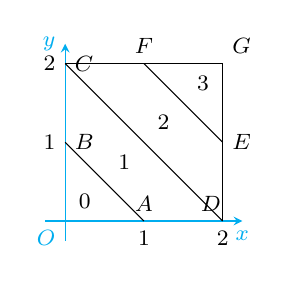
\begin{tikzpicture}[->,samples=100,>=stealth,domain=-1:1,font=\footnotesize]
                \coordinate (xMin) at (-0.25,0);
                \coordinate (xMax) at (2.25,0);
                \coordinate (yMin) at (0,-0.25);
                \coordinate (yMax) at (0,2.25);
                \draw[->,cyan] (xMin)--(0,0) node [below left] {$O$}--(xMax) node[below] {$x$};
                \draw[->,cyan] (yMin)--(yMax) node [left] {$y$};
                \draw[-] (2,0)--(2,2)--(0,2);
                \draw[-] (1,0)--(0,1);
                \draw[-] (2,0)--(0,2);
                \draw[-] (2,1)--(1,2);
                \node at (0.25,0.25) {$0$};
                \node at (0.75,0.75) {$1$};
                \node at (1.25,1.25) {$2$};
                \node at (1.75,1.75) {$3$};
                \node at (1,0) [below] {$1$};
                \node at (2,0) [below] {$2$};
                \node at (1,0) [above] {$A$};
                \node at (2,0) [above] {$D~~~$};
                \node at (0,1) [left] {$1$};
                \node at (0,1) [right] {$B$};
                \node at (0,2) [left] {$2$};
                \node at (0,2) [right] {$C$};
                \node at (2,1) [right] {$E$};
                \node at (1,2) [above] {$F$};
                \node at (2,2) [above right] {$G$};
            \end{tikzpicture}
        }
        \caption{}
    \end{figure}
\end{solution}

% \begin{example}
%     设函数 $f(x,y)$ 在点 $(0,0)$ 的某个领域内具有二阶连续偏导数,求极限 $$\lim_{\rho\to0^+}\dfrac{1}{\rho^4}\iint\limits_{x^2+y^2\leqslant \rho^2}[f(x,y)-f(0,0)]\dd x\dd y.$$
% \end{example}

\begin{example}
    设函数 $f(x)$ 满足
    $$f(x)=x^2+x\int_{0}^{x^2}f\qty(x^2-t)\dd t+\iint\limits_Df(xy)\dd x\dd y$$
    其中 $D$ 是以 $(-1,-1),~(1,-1),~(1,1)$ 为顶点的三角形,且 $f(1)=0$,求 $\displaystyle\int_{0}^{1}f(x)\dd x.$
\end{example}
\begin{solution}
    令 $\displaystyle\iint\limits_D f(xy)\dd x\dd y=A$,那么 $\displaystyle f(x)=x^2+x\int_{0}^{x^2}f\qty(x^2-t)\dd t+A$,
    将 $x$ 替换为 $xy$ 得 $$f(xy)=x^2y^2+xy\int_{0}^{x^2y^2}f\qty(x^2y^2-t)\dd t+A\Rightarrow f(xy)=x^2y^2+xy\int_{0}^{x^2y^2}f(u)\dd u+A$$
    % 并令 $u=x^2y^2-t$,那么 $\displaystyle\int_{0}^{x^2y^2}f\qty(x^2y^2-t)\dd t=\int_{0}^{x^2y^2}f(u)\dd u$,故上式转为
    % $$f(xy)=x^2y^2+xy\int_{0}^{x^2y^2}f(u)\dd u+A$$
    对等式两边二重积分得 $$A=\iint\limits_D x^2y^2\dd x\dd y+\iint\limits_D\qty[xy\int_{0}^{x^2y^2}f(u)\dd u]\dd x\dd y+A\iint\limits_D \dd x\dd y$$
    其中 $\displaystyle\iint\limits_D x^2y^2\dd x\dd y=\int_{-1}^{1}x^2\dd x\int_{-1}^{x}y^2\dd y=\dfrac{2}{9},~\iint\limits_D \dd x\dd y=2$,
    作 $y=-x$,将 $D$ 划分为关于 $x$ 轴对称的 $D_1$ 和关于 $y$ 轴对称的 $D_2$,并令函数 $\displaystyle g(x,y)=\int_{0}^{x^2y^2}f(u)\dd u$,关于 $x$ 和 $y$ 都是奇函数,利用二重积分的对称性知
    $$\iint\limits_D g(x,y)\dd x\dd y=\iint\limits_{D_1}g(x,y)\dd x\dd y+\iint\limits_{D_2}g(x,y)\dd x\dd y=0$$
    故 $A=-\dfrac{2}{9}$,又由已知条件 $f(0)=1$,那么
    $$0=1+\int_{0}^{1}f(1-t)\dd t-\dfrac{2}{9}\Rightarrow\int_{0}^{1}f(x)\dd x=-\dfrac{7}{9}.$$
\end{solution}

\begin{example}
    求积分 $I=\displaystyle\int_{-1}^{1}\dd z\iint\limits_{x^2+y^2\leqslant 1-z^2}\dfrac{\qty(\cos x+\sin y+\sqrt{3}z)^2}{\qty(x^2+y^2+z^2)^2+1}\dd x\dd y$.
\end{example}
\begin{solution}
    记 $\Omega=\qty{(x,y,z)\mid x^2+y^2+z^2\leqslant 1}$,由对称性得
    \begin{flalign*}
        I & =\iiint\limits_\Omega\dfrac{\qty(\cos x+\sin y+\sqrt{3}z)^2}{\qty(x^2+y^2+z^2)^2+1}\dd V=\iiint\limits_\Omega\dfrac{\qty(\cos x+\sin y)^2+3z^2+2\sqrt{3}z(\cos x+\sin y)}{\qty(x^2+y^2+z^2)^2+1}\dd V                  \\
          & =\iiint\limits_\Omega\dfrac{(\cos x+\sin y)^2+3z^2}{\qty(x^2+y^2+z^2)^2+1}\dd V=\iiint\limits_\Omega\dfrac{(\cos x+\sin y)^2}{\qty(x^2+y^2+z^2)^2+1}\dd V+3\iiint\limits_\Omega\dfrac{z^2}{\qty(x^2+y^2+z^2)^2+1}\dd V \\
          & =\iiint\limits_\Omega\dfrac{\cos^2x+\sin^2y}{\qty(x^2+y^2+z^2)^2+1}\dd V+3\iiint\limits_\Omega\dfrac{z^2}{\qty(x^2+y^2+z^2)^2+1}\dd V                                                                                  \\
          & =\dfrac{1}{2}\iiint\limits_\Omega\dfrac{\cos^2x+\cos^2y+\sin^2x+\sin^2y}{\qty(x^2+y^2+z^2)+1}\dd V+3\iiint\limits_\Omega\dfrac{z^2}{\qty(x^2+y^2+z^2)^2+1}\dd V                                                        \\
          & =\iiint\limits_\Omega\dfrac{\dd V}{\qty(x^2+y^2+z^2)^2+1}+3\iiint\limits_\Omega\dfrac{z^2}{\qty(x^2+y^2+z^2)^2+1}\dd V                                                                                                 \\
          & =\int_{0}^{2\pi}\dd \theta\int_{0}^{\pi}\sin\varphi\dd \varphi\int_{0}^{1}\dfrac{r^2}{r^4+1}\dd r+3\int_{0}^{2\pi}\dd \theta\int_{0}^{\pi}\sin\varphi\cos^2\varphi\dd\varphi\int_{0}^{1}\dfrac{r^4}{r^4+1}\dd r        \\
          & =4\pi\int_{0}^{1}\dfrac{r^4+r^2}{r^4+1}\dd r=4\pi+\sqrt{2}\pi\ln\qty(3-2\sqrt{2})
    \end{flalign*}
    其中 $\displaystyle\int_{0}^{1}\dfrac{r^4+r^2}{r^4+1}\dd r=\int_{0}^{1}\dfrac{r^4+1+r^2-1}{r^4+1}\dd r=\int_{0}^{1}\dd r+\int_{0}^{1}\dfrac{r^2-1}{r^4+1}\dd r$,
    \begin{flalign*}
        \int\dfrac{r^2-1}{r^4+1}\dd r =\int\dfrac{1-\dfrac{1}{r^2}}{\qty(r+\dfrac{1}{r})^2-2}\dd r\xlongequal{r+\frac{1}{r}=t}\int\dfrac{\dd t}{\qty(t-\sqrt{2})\qty(t+\sqrt{2})} =\dfrac{1}{2\sqrt{2}}\ln\qty|\dfrac{t-\sqrt{2}}{t+\sqrt{2}}|+C=\dfrac{1}{2\sqrt{2}}\ln\qty|\dfrac{r+\dfrac{1}{r}-\sqrt{2}}{r+\dfrac{1}{r}+\sqrt{2}}|+C.
    \end{flalign*}
\end{solution}

\subsection{反常二重积分与含参变量积分}

\subsubsection{反常二重积分}

\begin{definition}[反常二重积分]
    若 $\displaystyle\iint\limits_D f(x,y)\dd \sigma$ 为反常积分,则取 $D'$,使 $D'\subset D$ 并且 $\displaystyle\iint\limits_{D'}f(x,y)\dd \sigma$ 为一般的二重积分,则
    $$\iint\limits_D f(x,y)\dd \sigma=\lim_{D'\to D}\iint\limits_{D'}f(x,y)\dd \sigma$$
    事实上,当反常二重积分可积时,其计算方法与一般二重积分基本相同.
\end{definition}

\begin{example}
    计算二重积分 $\displaystyle I=\iint\limits_{\frac{x^2}{a^2}+\frac{y^2}{b^2}\geqslant 1}\mathrm{e}^{-\qty(\frac{x^2}{a^2}+\frac{y^2}{b^2})}\dd x\dd y.$
\end{example}
\begin{solution}
    令 $x=ar\cos\theta,~y=br\sin\theta$,那么 $\dd x\dd y=abr\dd r\dd \theta$,故
    \begin{flalign*}
        I=ab\iint\limits_{\substack{0\leqslant \theta\leqslant 2\pi \\1\leqslant r\leqslant +\infty}}\mathrm{e}^{-r^2}r\dd r\dd \theta=ab\int_{0}^{2\pi}\dd \theta\int_{1}^{+\infty}r\mathrm{e}^{-r^2}\dd r=\dfrac{\pi ab}{\mathrm{e}}.
    \end{flalign*}
\end{solution}

\begin{example}
    求不定积分 $\displaystyle\int_{0}^{+\infty}\dfrac{1-\mathrm{e}^{-ax}}{x}\cos x\dd x,~a>0.$
\end{example}
\begin{solution}
    注意到 $$\int_{a}^{b}\mathrm{e}^{-yx}\cos x\dd y=-\dfrac{\cos x}{x}\int_{a}^{b}\mathrm{e}^{-yx}\dd (-yx)=-\dfrac{\cos x}{x}\qty(\mathrm{e}^{-yx})\biggl |_{y=a}^{y=b}=-\dfrac{\mathrm{e}^{-bx}-\mathrm{e}^{-ax}}{x}\cos x$$
    所以 $\displaystyle\int_{0}^{a}\mathrm{e}^{-yx}\cos x\dd y=\dfrac{1-\mathrm{e}^{-ax}}{x}\cos x$,交换积分次序可知: $\displaystyle\text{原式}=\int_{0}^{a}\dd y\int_{0}^{+\infty}\mathrm{e}^{-yx}\cos x\dd x$
    \begin{flalign*}
         & \int_{0}^{+\infty}\mathrm{e}^{-yx}\cos x\dd x=\int_{0}^{+\infty}\mathrm{e}^{-yx}\dd (\sin x)=\mathrm{e}^{-yx}\sin\biggl |_{x=0}^{x=+\infty}-\int_{0}^{+\infty}\sin x\dd \qty(\mathrm{e}^{-yx})          \\
         & =-y\int_{0}^{+\infty}\mathrm{e}^{-yx}\sin x\dd x=y\int_{0}^{+\infty}\mathrm{e}^{-yx}\dd (\cos x)=y\qty(\mathrm{e}^{-yx}\cos x\biggl |_{x=0}^{x=+\infty}+y\int_{0}^{+\infty}\cos x\mathrm{e}^{-yx}\dd x) \\
         & \Rightarrow \int_{0}^{+\infty}\mathrm{e}^{-yx}\cos x\dd x=\dfrac{y}{1+y^2}
    \end{flalign*}
    故 $$\int_{0}^{+\infty}\dfrac{1-\mathrm{e}^{-ax}}{x}\cos x\dd x=\int_{0}^{a}\dfrac{y}{1+y^2}\dd y=\dfrac{1}{2}\ln\qty(1+y^2)\biggl |_0^a=\dfrac{1}{2}\ln\qty(1+a^2).$$
\end{solution}

\begin{example}
    计算 $\displaystyle\int_0^{+\infty}\frac{\sin(5x)-\sin(3x)}{x}\mathrm{e}^{-2x}\dd x.$
\end{example}
\begin{solution}
    注意到 $\displaystyle\frac{\sin(5x)-\sin(3x)}{x}=\int_3^5\cos(xy)\dd y$,$\displaystyle\text{所以原式=}\int_0^{+\infty}\dd x\int_3^5\mathrm{e}^{-2x}\cos(xy)\dd y$,\\
    由于 $|\mathrm{e}^{-2x}\cos(xy)|\leqslant \mathrm{e}^{-2x}$,且 $\displaystyle\int_0^{+\infty}\mathrm{e}^{-2x}\dd x$ 收敛,
    所以 $\displaystyle \int_3^5\cos(xy)\dd x$ 关于 $y\in[3,5]$ 一致收敛,再结合 $\mathrm{e}^{-2x}\cos(xy)$ 为 $[0,+\infty)\times[3,5]$ 上的连续函数,所以
    \begin{flalign*}
        I & =\int_0^{+\infty}\dd x\int_3^5\mathrm{e}^{-2x}\cos(xy)\dd y=\int_3^5\dd y\int_0^{+\infty}\mathrm{e}^{-2x}\cos(xy)\dd x \\
          & =\int_3^5\frac{\mathrm{e}^{-2x}}{4+y^2}\bigl[-2\cos(xy)+y\sin(xy)\bigr]_0^{+\infty}\dd y=2\int_3^5\frac{\dd y}{4+y^2}  \\
          & =\arctan\frac{y}{2}\biggl |_3^5=\arctan\frac{5}{2}-\arctan\frac{3}{2}=\arctan\frac{4}{19}.
    \end{flalign*}
\end{solution}

\begin{example}
    计算 $\displaystyle I=\iint\limits_D\mathrm{e}^{-\left(x^2+y^2\right)}\cos\left(x^2+y^2\right)\dd x\dd y$,其中 $D$ 是全平面.
\end{example}
\begin{solution}
    用极坐标,化为先 $\theta$ 后 $\rho$ 次序的二次积分,
    \begin{flalign*}
        I=\int_0^{+\infty}\dd \rho\int_0^{2\pi}\rho\mathrm{e}^{-\rho^2}\cos\rho^2\dd \theta
        =2\pi\int_0^{+\infty}\rho\mathrm{e}^{-\rho^2}\cos\rho^2\dd \rho.
    \end{flalign*}
    其中,
    \begin{flalign*}
        \int\rho\mathrm{e}^{-\rho^2}\cos\rho^2\dd \rho
         & =\int\frac{4\rho\cos\rho^2}{4\mathrm{e}^{\rho^2}}\dd \rho
        =\int\frac{2\rho\cos\rho^2+2\rho\sin\rho^2-2\rho\left(\sin\rho^2-\cos\rho^2\right)}{4\mathrm{e}^{\rho^2}}\dd \rho                                                         \\
         & =\int\frac{\left(2\rho\cos\rho^2+2\rho\sin\rho^2\right)4\mathrm{e}^{\rho^2}-8\rho\mathrm{e}^{\rho^2}\left(\sin\rho^2-\cos\rho^2\right)}{16\mathrm{e}^{\rho^2}}\dd \rho \\
         & =\int\dd \left(\frac{\sin\rho^2-\cos\rho^2}{4\mathrm{e}^{\rho^2}}\right)
        =\frac{\sin\rho^2-\cos\rho^2}{4\mathrm{e}^{\rho^2}}+C
    \end{flalign*}
    所以,$\displaystyle I=
        2\pi\cdot\left .\frac{\sin\rho^2-\cos\rho^2}{4\mathrm{e}^{\rho^2}}\right |_0^{+\infty}
        =\frac{\pi}{2}$.
\end{solution}

\begin{example}
    计算 $\displaystyle\iint\limits_D\dfrac{x^2+y^2-2}{\qty(x^2+y^2)^{\frac{5}{2}}}\dd x\dd y$,其中 $D:x^2+y^2\geqslant 2,x\leqslant 1.$
\end{example}
\begin{solution}
    注意到 $ D $ 关于 $ x $ 轴对称,且被积函数关于 $ y $ 变量为偶函数,记 $ x $ 轴上方部分积分区域为 $ D_{1}$,
    令 $ x=r \cos \theta, y=r \sin \theta $,则在极坐标下,$ D_{1} $ 可以描述为两部分,如图 \ref{dd1d2} 所示,记作
    $$D_{1}^{\prime}:\frac{\pi}{4} \leqslant \theta \leqslant \frac{\pi}{2}, \sqrt{2} \leqslant r \leqslant \sec \theta,~D_{2}^{\prime}:\frac{\pi}{2} \leqslant \theta \leqslant \pi, \sqrt{2} \leqslant r \leqslant+\infty$$
    \begin{minipage}{.38\linewidth}
        \begin{figure}[H]
            \centering
            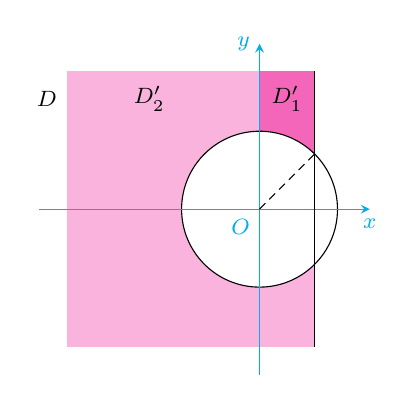
\begin{tikzpicture}[samples=100,>=stealth,font=\footnotesize,scale=0.7]
                \coordinate (xMin) at (-4,0);
                \coordinate (xMax) at (2,0);
                \coordinate (yMin) at (0,-3);
                \coordinate (yMax) at (0,3);
                \fill[magenta!30] (-3.5,-2.5)--(1,-2.5)--(1,2.5)--(-3.5,2.5)--cycle;
                \fill[magenta!60] (0,0)--(1,0)--(1,2.5)--(0,2.5)--cycle;
                \filldraw[fill=white](0,0) circle ({sqrt(2)});
                \draw[->,cyan] (xMin)--(0,0) node [below left] {$O$}--(xMax) node[below] {$x$};
                \draw[->,cyan] (yMin)--(yMax) node [left] {$y$};
                \draw[-] (1,-2.5)--(1,2.5);
                \draw[densely dashed] (0,0)--(1,1);
                \node[left] at (-3.5,2) {$D$};
                \node at (0.5,2) {$D_1'$};
                \node at (-2,2) {$D_2'$};
            \end{tikzpicture}
            \caption{}
            \label{dd1d2}
        \end{figure}
    \end{minipage}
    \hfill
    \begin{minipage}{.58\linewidth}
        \begin{flalign*}
            I & =2\int_{\frac{\pi}{4}}^{\frac{\pi}{2}}\dd \theta \int_{\sqrt{2}}^{\sec\theta}\dfrac{r^2-2}{r^5}r\dd r+2\int_{\frac{\pi}{2}}^{\pi}\dd \theta\int_{\sqrt{2}}^{+\infty}\dfrac{r^2-2}{r^5}r\dd r                                   \\
              & =2 \int_{\frac{\pi}{4}}^{\frac{\pi}{2}}\left(\frac{2}{3 r^{3}}-\frac{1}{r}\right)_{\sqrt{2}}^{\sec \theta} \dd  \theta+2 \int_{\frac{\pi}{2}}^{\pi}\left(\frac{2}{3 r^{3}}-\frac{1}{r}\right)_{\sqrt{2}}^{+\infty} \dd  \theta \\
              & =2 \int_{\frac{\pi}{4}}^{\frac{\pi}{2}}\left(\frac{2 \cos ^{3} \theta}{3}-\cos \theta+\frac{\sqrt{2}}{3}\right) \dd  \theta+2 \int_{\frac{\pi}{2}}^{\pi} \frac{\sqrt{2}}{3} \dd  \theta                                        \\
              & =2\left[\frac{2}{3}\left(\sin \theta-\frac{\sin ^{3} \theta}{3}\right)-\sin \theta+\frac{\sqrt{2}}{3} \theta\right]_{\frac{\pi}{4}}^{\frac{\pi}{2}}+2 \cdot \frac{\pi}{3 \sqrt{2}}                                             \\
              & =2 \cdot\left(\frac{\pi}{3 \sqrt{2}}-\frac{5}{9}-\frac{\pi}{6 \sqrt{2}}+\frac{2 \sqrt{2}}{9}\right)+\frac{\sqrt{2}}{3} \pi=\frac{4 \sqrt{2}}{9}-\frac{10}{9}+\frac{\sqrt{2}}{2} \pi
        \end{flalign*}
    \end{minipage}
\end{solution}

\begin{example}
    计算 $\displaystyle I=\int_{-\infty}^{+\infty}\int_{-\infty}^{+\infty}\min\qty{x,y}\e ^{-\qty(x^2+y^2)}\dd x\dd y.$
\end{example}
\begin{solution}
    由题意
    \begin{flalign*}
        I & =\int_{-\frac{3\pi}{4}}^{\frac{\pi}{4}}\dd \theta\int_{0}^{+\infty}r\sin\theta\e ^{-r^2}r\dd r+\int_{\frac{\pi}{4}}^{\frac{5\pi}{4}}\dd \theta\int_{0}^{+\infty}r\cos\theta\e ^{-r^2}r\dd r=-2\sqrt{2}\int_{0}^{+\infty}r^2\e ^{-r^2}\dd r \\
          & =-\sqrt{2}\cdot 2\int_{0}^{+\infty}r^2\e ^{-r^2}\dd r=-\sqrt{2}\Gamma\qty(\dfrac{3}{2})=-\sqrt{2}\Gamma\qty(\dfrac{1}{2})=-\dfrac{\sqrt{2\pi}}{2}.
    \end{flalign*}
\end{solution}

\subsubsection{含参变量积分}

含参变量积分是指在积分运算中,被积函数中包含一个或多个参数的情况. 这种情况下,参数被视为常数,而不是变量,因此在积分时需要将参数视为常数处理.

\begin{theorem}[含参变量积分求导公式]
    设 $f(t,x),f_x(t,x)$ 在 $R=[a,b]\times[p,q]$ 上连续,$\alpha(x),\beta(x)$ 为定义在 $[a,b]$ 上其值含于 $[p,q]$ 内的可微函数,则函数
    $$F(t,x)=\int_{\alpha(x)}^{\beta(x)}f(t,x)\dd t$$
    在 $[a,b]$ 上可微,且
    $$F'(t,x)=\dv{x}\int_{\alpha(x)}^{\beta(x)}f(t,x)\dd t=\int_{\alpha(x)}^{\beta(x)}f_x(t,x)\dd t+f[\beta(x),x]\beta'(x)-f[\alpha(x),x]\alpha'(x).$$
    \index{含参变量积分求导公式}
\end{theorem}

\begin{example}
    已知 $\displaystyle F(x)=\int_{\sin x}^{\cos x}\mathrm{e}^{\qty(xt+x^2)}\dd t$,求 $\displaystyle\dv{F(x)}{x}\biggl |_{x=0}.$
\end{example}
\begin{solution}
    \textbf{法一: }由含参变量积分求导公式,有
    \begin{flalign*}
        I & =\dv{x}\int_{\sin x}^{\cos x}\mathrm{e}^{\qty(xt+x^2)}\dd t=\qty[\int_{\sin x}^{\cos x}(t+2x)\mathrm{e}^{\qty(xt+x^2)}\dd t-\sin x\mathrm{e}^{\qty(x\cos x+x^2)}-\cos x\mathrm{e}^{\qty(x\sin x+x^2)}]_{x=0} \\
          & =\int_{0}^{1}t\dd t-1=-\dfrac{1}{2}
    \end{flalign*}
    \textbf{法二: }由题意,
    \begin{flalign*}
        F(x)=\int_{\sin x}^{\cos x}\mathrm{e}^{\qty(xt+x^2)}\dd t=\mathrm{e}^{x^2}\int_{\sin x}^{\cos x}\mathrm{e}^{xt}\dd t\xlongequal[]{xt=u}\dfrac{\mathrm{e}^{x^2}}{x}\int_{x\sin x}^{x\cos x}\mathrm{e}^u\dd u=\dfrac{\mathrm{e}^{x^2}}{x}\qty(\mathrm{e}^{x\cos x}-\mathrm{e}^{x\sin x})
    \end{flalign*}
    其中 $x\neq0$,且 $F(0)=1$,所以考虑导数定义式,有
    \begin{flalign*}
        \dv{F(x)}{x}\biggl |_{x=0}=\lim_{x\to0}\dfrac{F(x)-F(0)}{x-0}=\lim_{x\to0}\dfrac{\dfrac{\mathrm{e}^{x^2}}{x}\qty(\mathrm{e}^{x\cos x}-\mathrm{e}^{x\sin x})-1}{x}=\lim_{x\to0}\dfrac{\mathrm{e}^{x^2}\qty(\mathrm{e}^{x\cos x}-\mathrm{e}^{x\sin x})-x}{x^2}
    \end{flalign*}
    由 $\mathrm{e}^x=1+x+\dfrac{x^2}{2}+o\qty(x^2),~\cos x=1-\dfrac{x^2}{2}+o\qty(x^2),~\sin x=x+o(x)$ 得
    \begin{flalign*}
        \mathrm{e}^{x\cos x} & =1+x\cos x+\dfrac{1}{2}(x\cos x)^2+o\qty((x\cos x)^2)                                              \\
                             & =1+x\qty(1-\dfrac{x^2}{2}+o\qty(x^2))+\dfrac{x^2}{2}\qty(1-\dfrac{x^2}{2}+o\qty(x^2))^2+o\qty(x^2) \\
                             & =1+x+\dfrac{x^2}{2}+o\qty(x^2)                                                                     \\
        \mathrm{e}^{x\sin x} & =1+x\sin x+(x\sin x)^2+o\qty((x\sin x)^2)=1+x^2+o\qty(x^2)                                         \\
        \mathrm{e}^{x^2}     & =1+x^2+o\qty(x^2)
    \end{flalign*}
    将上述展开式代入原极限式,化简最终求得原极限等于 $-\dfrac{1}{2}.$
\end{solution}

\begin{example}
    设 $f(x)$ 为连续函数,$t>0$,区域 $\Omega$ 是由抛物面 $z=x^2+y^2$ 和球面 $x^2+y^2+z^2=t^2~ (t>0)$ 所围成的部分,定义三重积分 $\displaystyle F(t)=\iiint\limits_{\Omega}f\qty(x^2+y^2+z^2)\dd v$,求 $F'(t).$
\end{example}
\begin{solution}
    利用柱坐标系,令 $\begin{cases}
            x=r\cos\theta \\ y=r\sin\theta\\ z=z
        \end{cases}$,则由 $\begin{cases}
            z=x^2+y^2 \\ x^2+y^2+z^2=t^2
        \end{cases}$ 联立得 $z^2=z+t^2$,解得 $z=\dfrac{\sqrt{1+4t^2}-1}{2}:=b^2(t)$,
    于是区域 $\Omega$ 在 $xOy$ 平面上的投影区域为 $D_{xy}:x^2+y^2\leqslant b^2(t)$,从而
    $$F(t)=\int_{0}^{2\pi}\dd \theta\int_{0}^{b(t)}r\dd r\int_{r^2}^{\sqrt{t^2-r^2}}f\qty(r^2+z^2)\dd z=2\pi\int_{0}^{b(t)}r\qty[\int_{r^2}^{\sqrt{t^2-r^2}}f\qty(r^2+z^2)\dd z]\dd r$$
    记 $\displaystyle g(t,r)=r\qty[\int_{r^2}^{\sqrt{t^2-r^2}}f\qty(r^2+z^2)\dd z]$,则由 $f(x)$ 的连续知, $g(t,r)$ 及 $\displaystyle\pdv{g(t,r)}{r}$ 连续,
    于是由含参变量积分的求导公式,得
    \begin{flalign*}
        F'(t) & =2\pi\qty[\int_{0}^{b(t)}\pdv{g}{t}\dd r+g(t,b(t))\cdot b'(t)]                                                                             \\
              & =2\pi\qty[\int_{0}^{b(t)}rf\qty(t^2)\dfrac{t}{\sqrt{t^2-r^2}}\dd r+b(t)\int_{b^2(t)}^{\sqrt{t^2-b^2(t)}}f\qty(b^2(t)+z^2)\dd z\cdot b'(t)] \\
              & =2\pi tf\qty(t^2)\int_{0}^{b(t)}\dfrac{r}{\sqrt{t^2-r^2}}\dd r=-\pi tf\qty(t^2)\int_{0}^{b(t)}\dfrac{\dd \qty(t^2-r^2)}{\sqrt{t^2-r^2}}    \\
              & =2\pi tf\qty(t^2)\qty(t-\sqrt{t^2-b^2(t)})=2\pi tf\qty(t^2)\qty(t-b^2(t))=\pi t\qty f(t^2)\qty(2t+1-\sqrt{1+4t^2}).
    \end{flalign*}
\end{solution}

\begin{example}\scriptsize\linespread{0.8}
    求 $\displaystyle \dv[n]{}{x}\qty[\int_0^x\mathrm{e}^{nt}\sum_{k=0}^{n-1}\dfrac{(x-t)^k}{k!}\dd t].$
\end{example}
\begin{solution}\scriptsize\linespread{0.8}
    记 $\displaystyle f_k(x)=\int_{0}^{x}\mathrm{e}^{nt}\dfrac{(x-t)^k}{k!}\dd t$,那么 $\displaystyle\dv{x}f_k(x)=\int_{0}^{x}\mathrm{e}^{nt}\dfrac{(x-t)^{k-1}}{(k-1)!}\dd t=f_{k-1}(x)$,于是
    $$f''_k(x)=f'_{k-1}(x)=f_{k-2}(x),~\cdots,~f_k^{(k)}(x)=f_0(x)$$
    由于 $\displaystyle f_0'(x)=\qty(\int_{0}^{x}\mathrm{e}^{nt}\dd t)'=\mathrm{e}^{nx},~f_0''(x)=n\mathrm{e}^{nx},~\cdots,~f_0^{(n)}(x)=n^{n-1}\mathrm{e}^{nx}$,所以
    \begin{flalign*}
        \dv[n]{}{x}\qty[\int_0^x\mathrm{e}^{nt}\sum_{k=0}^{n-1}\dfrac{(x-t)^k}{k!}\dd t]=\sum_{k=0}^{n-1}f_k^{(n)}(x)=f_0^{(n)}(x)+\sum_{k=1}^{n-1}\qty[f_k^{(k)}(x)]^{(n-k)}=\sum_{k=1}^{n}f_0^{(k)}(x)=\dfrac{1-n^n}{1-n}\mathrm{e}^{nx}.
    \end{flalign*}
\end{solution}

% \subsection{判断含参变量反常积分的一致收敛性}
% 
% \subsection{含参变量反常积分的极限与连续性}
% 
% \subsection{含参变量反常积分积分号下求导与积分号下求积分}

\subsection{重积分的积分中值定理}

\begin{theorem}[二重积分中值定理]
    若函数 $f(x,y)$ 在有界闭区域 $D$ 上连续,函数 $g(x,y)$ 在 $D$ 上可积且不变号,则 $\exists(\xi,\eta)\in D$,使得 $$\iint\limits_D f(x,y)g(x,y)\dd x\dd y=f(\xi,\eta)\iint\limits_D g(x,y)\dd x\dd y.$$
    \index{二重积分中值定理}
\end{theorem}

\begin{example}
    已知 $\displaystyle\lim_{x\to0^+}\dfrac{\displaystyle\int_{0}^{x}\dd v\int_{\ln(1+v)}^{v}\sin\qty(u^2)\dd u}{x^k}=c\neq0$,求 $c.$
\end{example}
\begin{errorSolution}
    记积分区域为 $D$,则由二重积分中值定理知,$\exists(\xi,\eta)\in D$,使得 $\displaystyle\iint\limits_D \sin\qty(u^2)\dd u\dd v=\sin\qty(\eta^2)\iint\limits_D \dd u\dd v$,下求 $D$ 的面积 $S$,
    记 $I_1=\dfrac{1}{2}x^2,~\displaystyle I_2=\int_{0}^{x}\ln(1+t)\dd t$,于是 $$I_2=\int_{0}^{x}\ln(1+t)\dd t=x\ln(1+x)-x+\ln(1+x)$$
    因此 $S=I_1-I_2=\dfrac{1}{2}x^2-x\ln(1+x)+x-\ln(1+x)$,故极限式化为
    $$\lim_{x\to0^+}\dfrac{x^2\qty[\dfrac{1}{2}x^2-x\ln(1+x)+x-\ln(1+x)]}{x^k}=\lim_{x\to0^+}\dfrac{x^2\qty[\dfrac{1}{2}x^2-x^2+\dfrac{1}{2}x^3+x-x+\dfrac{1}{2}x^2-\dfrac{1}{3}x^3+o\qty(x^3)]}{x^k}=\lim_{x\to0^+}\dfrac{\dfrac{x^5}{6}}{x^k}$$
    因为 $c\neq0$,所以分子与分母等阶,因此 $c=\dfrac{1}{6}.$\\
    \textbf{错因: }对二重积分中值定理内容了解不透彻,该定理说的是: 若函数 $f(x,y)$ 在有界闭区域 $D$ 上连续,函数 $g(x,y)$ 在 $D$ 上可积且不变号,则存在一点 $(\xi,\eta)\in D$,使得 $$\iint\limits_D f(x,y)g(x,y)\dd x\dd y=f(\xi,\eta)\iint\limits_D g(x,y)\dd x\dd y.$$
\end{errorSolution}
\begin{solution}
    \textbf{法一: }先使用 L'Hospital 法则,将二重积分转化为定积分,再使用积分中值定理,有
    $$\lim_{x\to0^+}\dfrac{\displaystyle\int_{0}^{x}\dd v\int_{\ln(1+v)}^{v}\sin\qty(u^2)\dd u}{x^k}\xlongequal{L'}\lim_{x\to0^+}\dfrac{\displaystyle\int_{\ln(1+x)}^{x}\sin\qty(u^2)\dd u}{kx^{k-1}}=\lim_{x\to0^+}\dfrac{\sin\xi^2[x-\ln(1+x)]}{kx^{k-1}}$$
    其中 $x\gets\ln(1+x)<\xi<x~~(x\to0^+)$,因此原极限等于 $\displaystyle\lim_{x\to0^+}\dfrac{\dfrac{1}{2}x^4}{kx^{k-1}}$,因此 $k=5,c=\dfrac{1}{10}.$\\
    \textbf{法二: }因为 $\sin \qty(u^2)$ 在积分区间内不变号,因此 $\displaystyle\int_{\ln(1+v)}^{v}\sin\qty(u^2)\dd u\sim\int_{\ln(1+v)}^{v}u^2\dd u$,又因为 $\ln(1+v)\sim v~~(v\to0^+)$,因此原极限等价为
    $$\lim_{x\to0^+}\dfrac{\displaystyle\int_{0}^{x}\dd v\int_{\ln(1+v)}^{v}\sin\qty(u^2)\dd u}{x^k}=\lim_{x\to0^+}\dfrac{\displaystyle\int_{0}^{x}[v-\ln(1+v)]\xi_v^2\dd v}{x^k}=\lim_{x\to0^+}\dfrac{\displaystyle \int_{0}^{x}\dfrac{1}{2}v^4\dd v}{x^k}=c$$
    因为 $c\neq0$,因此分子与分母等阶,即 $\displaystyle\lim_{x\to0^+}\dfrac{\dfrac{1}{2}\cdot\dfrac{1}{5}x^5}{x^k}=c\Rightarrow c=\dfrac{1}{10}.$
\end{solution}

\begin{example}
    设区域 $D$ 为 $x^2+y^2\leqslant r^2$,求极限 $\displaystyle\lim_{r\to0}\frac{1}{\pi r^2}\iint\limits_D\mathrm{e}^{x^2-y^2}\cos(x+y)\dd x\dd y.$
\end{example}
\begin{solution}
    由二重积分的积分中值定理知,$\displaystyle\exists(\xi,\eta)\in D$,使得
    $$\iint\limits_D\mathrm{e}^{x^2-y^2}\cos(x+y)\dd x\dd y=\pi r^2\cdot\mathrm{e}^{\xi^2-\eta^2}\cos(\xi+\eta)$$
    于是,$\displaystyle\lim_{r\to0}\frac{1}{\pi r^2}\iint\limits_D\mathrm{e}^{x^2-y^2}\cos(x+y)\dd x\dd y
        =\lim_{\xi,\eta\to0}\mathrm{e}^{\xi^2-\eta^2}\cos(\xi+\eta)=1$.
\end{solution}

\begin{example}[2009 南京工业大学]
    求极限 $\displaystyle\lim_{t\to0^+}\frac{1}{t^2}\int_0^t\dd x\int_0^{t-x}\mathrm{e}^{x^2+y^2}\dd y.$
\end{example}
\begin{solution}
    由二重积分的积分中值定理知,$\displaystyle\exists(\xi,\eta)\in \{(x,y)|0\leqslant x\leqslant t,0\leqslant y\leqslant t-x\}$,使得
    $$\int_0^t\dd x\int_0^{t-x}\mathrm{e}^{x^2+y^2}\dd y=\frac{t^2}{2}\mathrm{e}^{\xi^2+\eta^2}$$
    于是,$\displaystyle\lim_{t\to0^+}\frac{1}{t^2}\int_0^t\dd x\int_0^{t-x}\mathrm{e}^{x^2+y^2}\dd y
        =\frac{1}{2}\lim_{\xi,\eta\to0^+}\mathrm{e}^{\xi^2+\eta^2}=\frac{1}{2}$.
\end{solution}
\begin{example}[2016 年天津市 (理工)]
    设函数 $f(x,y)$ 在点 $(0,0)$ 的某个领域内连续,求 $\displaystyle\lim_{t\to0^+}\frac{F'(t)}{t}$
    其中 $$F(t)=\iint\limits_{x^2+y^2\leqslant t^2}f(x,y)\dd x\dd y.$$
\end{example}
\begin{solution}
    由二重积分的积分中值定理知,$\exists(\xi,\eta)\in x^2+y^2\leqslant t^2$,使得
    $$F(t)=\iint\limits_{x^2+y^2\leqslant t^2}f(x,y)\dd x\dd y=\pi t^2 f(\xi,\eta)$$
    于是,$\displaystyle\lim_{t\to0^+}\frac{F'(t)}{t}=\lim_{\xi,\eta\to0^+}\frac{2\pi tf(\xi,\eta)}{t}
        =2\pi tf(0,0)$.
\end{solution}

\begin{example}[第十届 “景润杯”]
    计算极限 $\displaystyle\lim_{R\to+\infty}\iint\limits_{D_R}\mathrm{e}^{-x}\arctan\dfrac{y}{x}\dd x\dd y$,其中 $D_R$ 是由 $x=R,y=0,y=\dfrac{2}{R}x-1$ 所围成.
\end{example}
\begin{solution}
    由二重积分的积分中值定理知,$\exists(\xi,\eta)\in D_R$,
    使得 $$\iint\limits_{D_R}\mathrm{e}^{-x}\arctan\dfrac{y}{x}\dd x\dd y=\mathrm{e}^{-\xi}\arctan\dfrac{\eta}{\xi}\iint\limits_{D_R}\dd x\dd y=\dfrac{R}{4}\mathrm{e}^{-\xi}\arctan\dfrac{\eta}{\xi}$$
    其中 $R\in\qty(\dfrac{R}{2},R),~\eta\in(0,1)$,故 \begin{flalign*}
        \qty|\iint\limits_{D_R}\mathrm{e}^{-x}\arctan\dfrac{y}{x}\dd x\dd y|=\mathrm{e}^{-\xi}\arctan\dfrac{\eta}{\xi}\iint\limits_{D_R}\dd x\dd y\leqslant \dfrac{R}{4}\mathrm{e}^{-\frac{R}{2}}\arctan \dfrac{\eta}{\xi}\to0~ (R\to+\infty)
    \end{flalign*}
    所以 $\displaystyle\lim_{R\to+\infty}\iint\limits_{D_R}\mathrm{e}^{-x}\arctan\dfrac{y}{x}\dd x\dd y=0.$
\end{solution}

\begin{example}
    证明: $$\dfrac{\pi\qty(R^2-r^2)}{R+K}\leqslant \iint\limits_{D}\dfrac{\dd \sigma}{\sqrt{(x-a)^2+(y-b)^2}}\leqslant \dfrac{\pi\qty(R^2-r^2)}{r-K}$$
    其中 $0<K=\sqrt{a^2+b^2}<r<R,~D:r^2\leqslant x^2+y^2\leqslant R^2.$
\end{example}
\begin{proof}[{\songti \textbf{证}}]
    函数 $f(x,y)=\dfrac{1}{\sqrt{(x-a)^2+(y-b)^2}}$ 在环形闭域 $D:r^2\leqslant x^2+y^2\leqslant R^2$ 上连续,则由积分中值定理知,存在 $P_0(\xi,\eta)\in D$,使
    $$\iint\limits_{D}\dfrac{\dd \sigma}{\sqrt{(x-a)^2+(y-b)^2}}=\dfrac{1}{\sqrt{(\xi-a)^2+(\eta-b)^2}}\iint\limits_D\dd \sigma=\dfrac{1}{\qty|P_0P_1|}\pi\qty(R^2-r^2)$$
    \begin{minipage}{.28\linewidth}
        \begin{figure}[H]
            \centering
            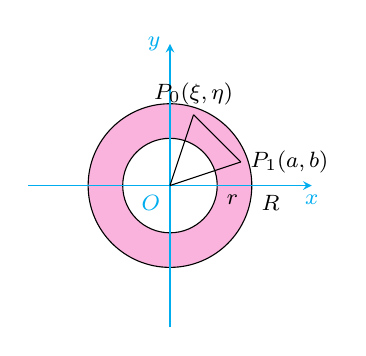
\begin{tikzpicture}[->,samples=100,>=stealth,scale=0.6,font=\footnotesize]
                \coordinate (xMin) at (-3,0);
                \coordinate (xMax) at (3,0);
                \coordinate (yMin) at (0,-3);
                \coordinate (yMax) at (0,3);
                \filldraw[fill=magenta!30](0,0) circle ({sqrt(3)});
                \filldraw[fill=white](0,0) circle ({sqrt(1)});
                \draw[->,cyan] (xMin)--(0,0) node [below left] {$O$}--(xMax) node[below] {$x$};
                \draw[->,cyan] (yMin)--(yMax) node [left] {$y$};
                \draw[-] (0,0)--(1.5,0.5) node[right] {$P_1(a,b)$};
                \draw[-] (0,0)--(0.5,1.5) node[above] {$P_0(\xi,\eta)$};
                \draw[-] (1.5,0.5)--(0.5,1.5);
                \node[below right] at (1,0) {$r$};
                \node[below right] at ({sqrt(3)},0) {$R$};
            \end{tikzpicture}
            \caption{}
            \label{RKr}
        \end{figure}
    \end{minipage}
    \hfill
    \begin{minipage}{.68\linewidth}
        由图 \ref{RKr} 知,$r\leqslant \qty|OP_0|\leqslant R$,且存在关系 $$r-K\leqslant \qty|OP_0|-\qty|OP_1|\leqslant|P_0P_1|\leqslant \qty|OP_1|+\qty|OP_0|\leqslant R+K$$
        所以 $$\dfrac{1}{R+K}\leqslant \dfrac{1}{\qty|P_0P_1|}\leqslant \dfrac{1}{r-K}$$
        代入上式得证不等式成立.
    \end{minipage}
\end{proof}

\subsection{重积分的应用}

\subsubsection{重积分在几何上的应用}

\begin{example}
    求球面 $x^2+y^2+z^2=4$ 和抛物面 $x^2+y^2=3z$ 所围的立体 (含在抛物面内部) $\Omega$ 的体积 $V$.
\end{example}
\begin{solution}
    \textbf{法一: }“先一后二”法,配合柱坐标
    \begin{flalign*}
        V=\iiint\limits_\Omega\dd v=\iint\limits_{D_{xy}}\dd x\dd y\int_{\frac{x^2+y^2}{3}}^{\sqrt{4-x^2-y^2}}\dd z=\int_{0}^{2\pi}\dd\theta\int_{0}^{\sqrt{3}}\rho\dd\rho\int_{\frac{\rho^2}{3}}^{\sqrt{4-\rho^2}}\dd z=\dfrac{19}{6}\pi.
    \end{flalign*}
    \textbf{法二: }“先二后一”法
    \begin{flalign*}
        V & =\iiint\limits_\Omega\dd v=\iiint\limits_{\Omega_1}\dd v+\iiint\limits_{\Omega_2}\dd v=\int_{0}^{1}\dd z\iint\limits_{D_{z_1}}\dd x\dd y+\int_{1}^{2}\dd z\iint\limits_{D_{z_2}}\dd x\dd y \\
          & =\int_{0}^{1}\pi\qty(\sqrt{3z})^2\dd z+\int_{1}^{2}\pi\qty(\sqrt{4-z^2})^2\dd z=\dfrac{19}{6}\pi.
    \end{flalign*}
    \textbf{法三: }利用球坐标
    \begin{flalign*}
        V=\iiint\limits_{\Omega}\dd v=\int_{0}^{2\pi}\dd \theta\int_{0}^{\frac{\pi}{3}}\dd \varphi\int_{0}^{2}\rho^2\sin\varphi\dd\rho+\int_{0}^{2\pi}\dd\theta\int_{\frac{\pi}{3}}^{\frac{\pi}{2}}\dd\varphi\int_{0}^{3\frac{\cos\varphi}{\sin^2\varphi}}\rho^2\sin\varphi\dd\rho=\dfrac{19}{6}\pi.
    \end{flalign*}
\end{solution}

\begin{example}
    求由方程 $\displaystyle\qty(\dfrac{x^2}{a^2}+\dfrac{y^2}{b^2})^2+\dfrac{z^4}{c^4}=z$ 所确定的曲面 $\varSigma$ 所围成空间立体 $\Omega$ 的体积,其中 $a,b,c$ 为正常数.
\end{example}
\begin{solution}
    利用广义球坐标公式 $\displaystyle \begin{cases}
            x = a\rho\cos\theta \sin\varphi \\
            y = b\rho\sin\theta \sin\varphi \\
            z = c\rho\cos\varphi
        \end{cases}$,于是 $\displaystyle \qty|\pdv{x,y,z}{\rho,\theta,\varphi}|=abc\rho^2\sin\varphi$,且
    $$\Omega'=\qty{(\rho,\theta,\varphi)\biggl | 0\leqslant \theta\leqslant 2\pi,0\leqslant \varphi\leqslant \dfrac{\pi}{2},0\leqslant \rho\leqslant \qty(\dfrac{c\cos \varphi}{\sin^4\varphi+\cos^4\varphi})^{\frac{1}{3}}}$$
    \begin{flalign*}
        V & =\iiint\limits_{\Omega'}\dd v=\int_{0}^{2\pi}\dd \theta\int_{0}^{\frac{\pi}{2}}\dd\varphi\int_{0}^{\qty(\frac{c\cos\varphi}{\sin^4\varphi+\cos^4\varphi})^{\frac{1}{3}}}abc\rho^2\sin\varphi\dd\rho=\dfrac{2}{3}\pi abc^2\int_{0}^{\frac{\pi}{2}}\dfrac{\sin\varphi\cos\varphi}{\sin^4\varphi+\cos^4\varphi}\dd\varphi \\
          & =\dfrac{2}{3}\pi abc^2\int_{0}^{\frac{\pi}{2}}\dfrac{\sin\varphi\cos\varphi}{\qty(\sin^2\varphi-\cos^2\varphi)+2\sin^2\varphi\cos^2\varphi}\dd \varphi=\dfrac{2}{3}\pi abc^2\int_{0}^{\frac{\pi}{2}}\dfrac{\sin\varphi\cos\varphi}{2\cos^4\varphi-2\cos^2\varphi+1}\dd \varphi                                         \\
          & \xlongequal[]{\cos^2\varphi=t}\dfrac{\pi}{3}abc^2\int_{0}^{1}\dfrac{\dd t}{2t^2-2t+1}=\dfrac{\pi}{3}abc^2\cdot\arctan(2t-1)\biggl |_0^1=\dfrac{\pi^2}{6}abc^2.
    \end{flalign*}
\end{solution}

\subsubsection{重积分在力学上的应用}

\begin{theorem}[物体的质量]
    若一物体占有区域 $V,\rho=\rho(x,y,z)$ 为它在点 $(x,y,z)$ 的密度,则该物体的质量等于 $\displaystyle M=\iiint\limits_V\rho\dd x\dd y\dd z.$
    \index{物体的质量}
\end{theorem}

\begin{example}
    设某物体所在的空间区域为 $\Omega:x^2+y^2+2z^2\leqslant x+y+2z$,密度函数为 $x^2+y^2+z^2$,求质量 $\displaystyle M=\iiint\limits_\Omega\qty(x^2+y^2+z^2)\dd x\dd y\dd z.$
\end{example}
\begin{solution}
    将 $x^2+y^2+2z^2\leqslant x+y+2z$ 化为 $$\qty(x-\dfrac{1}{2})^2+\qty(y-\dfrac{1}{2})^2+\qty[\sqrt{2}\qty(z-\dfrac{1}{2})]^2\leqslant 1$$
    于是 $\Omega$ 为一椭球,令 $u=x-\dfrac{1}{2},~v=y-\dfrac{1}{2},~w=\sqrt{2}\qty(z-\dfrac{1}{2})$,则区域 $\Omega\to\Omega':u^2+v^2+w^2\leqslant 1$,
    且 Jacobian 行列式 $\displaystyle J=\pdv{(x,y,z)}{(u,v,w)}=\dfrac{1}{\displaystyle \pdv{(u,v,w)}{(x,y,z)}}=\dfrac{1}{\begin{vmatrix}
                1 & 0 & 0        \\
                0 & 1 & 0        \\
                0 & 0 & \sqrt{2}
            \end{vmatrix}}=\dfrac{1}{\sqrt{2}}$,于是
    \begin{flalign*}
        M & =\iiint\limits_\Omega\qty(x^2+y^2+z^2)\dd x\dd y\dd z=\dfrac{1}{\sqrt{2}}\iiint\limits_{\Omega'}\qty[\qty(u+\dfrac{1}{2})^2+\qty(v+\dfrac{1}{2})^2+\qty(\dfrac{w}{\sqrt{2}}+\dfrac{1}{2})^2]\dd u\dd v\dd w                                          \\
          & =\dfrac{1}{\sqrt{2}}\iiint\limits_{\Omega' }\qty(u^2+v^2+\dfrac{w^2}{2})\dd u\dd v\dd w=\dfrac{1}{\sqrt{2}}\iiint\limits_{\Omega'}\qty(u+v+\dfrac{w}{\sqrt{2}})\dd u\dd v\dd w+\dfrac{1}{\sqrt{2}}\iiint\limits_{\Omega'}\dfrac{3}{4}\dd u\dd v\dd w \\
          & =\dfrac{1}{\sqrt{2}}\iiint\limits_{\Omega' }\qty(u^2+v^2+\dfrac{w^2}{2})\dd u\dd v\dd w+0+\dfrac{1}{\sqrt{2}}\cdot\dfrac{3}{4}\cdot\dfrac{4\pi}{3}
    \end{flalign*}
    记 $\displaystyle I=\iiint\limits_{\Omega'}\qty(u^2+v^2+\dfrac{w^2}{2})\dd u\dd v\dd w$,则
    $$I=\int_{0}^{2\pi}\dd \theta\int_{0}^{\pi}\sin\varphi\dd \varphi\int_{0}^{1}\rho^4\dd \rho=\dfrac{4\pi}{5}$$
    由对称性知,$\displaystyle\iiint\limits_{\Omega'}u^2\dd u\dd v\dd w=\iiint\limits_{\Omega'}v^2\dd u\dd v\dd w=\iiint\limits_{\Omega'}w^2\dd u\dd v\dd w=\dfrac{I}{3}=\dfrac{4\pi}{15}$,
    故 $$M=\dfrac{1}{\sqrt{2}}\qty(\dfrac{4\pi}{15}+\dfrac{4\pi}{15}+\dfrac{1}{2}\cdot\dfrac{4\pi}{15})+\dfrac{\pi}{\sqrt{2}}=\dfrac{5}{6}\sqrt{2}\pi.$$
\end{solution}

\begin{theorem}[物体的质心]
    物体的质心坐标 $(x_0,y_0,z_0)$ 按下列公式来计算
    $$\begin{cases}
            x_0=\dfrac{1}{M}\displaystyle\iiint\limits_V\rho x\dd x\dd y\dd z, \\
            y_0=\dfrac{1}{M}\displaystyle\iiint\limits_V\rho y\dd x\dd y\dd z, \\
            z_0=\dfrac{1}{M}\displaystyle\iiint\limits_V\rho z\dd x\dd y\dd z, \\
        \end{cases}$$
    若物体是均匀的,则 $\rho=1.$
    \index{物体的质心}
\end{theorem}

\begin{example}
    求以下列曲面为界的均匀物体的质心坐标.
    \setcounter{magicrownumbers}{0}
    \begin{table}[H]
        \centering
        \begin{tabular}{l | l}
            (\rownumber{}) $\dfrac{x^2}{a^2}+\dfrac{y^2}{b^2}=\dfrac{z^2}{c^2},~z=c.$ & (\rownumber{}) $\dfrac{x^2}{a^2}+\dfrac{y^2}{b^2}+\dfrac{z^2}{c^2}=1,~x,y,z\geqslant 0.$ \\
        \end{tabular}
    \end{table}
\end{example}
\begin{solution}
    \begin{enumerate}[label=(\arabic{*})]
        \item 令 $x=ar\cos \theta,y=br\sin\theta,z=z$,则质量为 $$M=\iiint\limits_V\dd x\dd y\dd z=ab\int_{0}^{c}\dd z\int_{0}^{2\pi}\dd \theta\int_{0}^{\frac{z}{c}}r\dd r=\dfrac{\pi abc }{3}$$
              设质心坐标为 $(x_0,y_0,z_0)$,由对称性知,$x_0=y_0=0$,而 $$z_0=\dfrac{1}{M}\iiint\limits_V z\dd x\dd y\dd z=\dfrac{1}{M}\int_{0}^{c}z\dd z\int_{0}^{2\pi}\dd \theta\int_{0}^{\frac{z}{c}}r\dd r=\dfrac{3c}{4}$$
              于是质心坐标为 $\qty(0,0,\dfrac{3c}{4})$.
        \item 令 $x=a\rho \sin\varphi\cos \theta,~y=b\rho\sin\varphi\cos\theta,~z=c\rho\cos\varphi$,则质量为
              $$M=abc\int_{0}^{\frac{\pi}{2}}\dd \theta\int_{0}^{\frac{\pi}{2}}\sin\varphi\dd \varphi\int_{0}^{1}\rho^2\dd \rho=\dfrac{\pi abc}{6}$$
              设质心坐标为 $(x_0,y_0,z_0)$,那么
              \begin{flalign*}
                  x_0=\dfrac{1}{M}\iiint\limits_Vx\dd x\dd y\dd z=\dfrac{a^2bc}{M}\int_{0}^{\frac{\pi}{2}}\cos\theta\dd \theta\int_{0}^{\frac{\pi}{2}}\sin^2\varphi\dd \varphi\int_{0}^{1}\rho^3\dd \rho=\dfrac{3}{8}a
              \end{flalign*}
              由对称性知质心坐标为 $\qty(\dfrac{3}{8}a,\dfrac{3}{8}b,\dfrac{3}{8}c).$
    \end{enumerate}
\end{solution}

\begin{theorem}[转动惯量]
    积分 $$I_{xy}=\iiint\limits_V\rho z^2\dd x\dd y\dd z,~I_{yz}=\iiint\limits_V\rho x^2\dd x\dd y\dd z,~I_{zx}=\iiint\limits_V\rho y^2\dd x\dd y\dd z$$
    分别称为物体对坐标平面的转动惯量;
    $$I_l=\iiint\limits_V \rho r^2\dd x\dd y\dd z$$
    其中 $r$ 为物体各点 $(x,y,z)$ 与轴 $l$ 的距离,特别地,对于坐标轴 $Ox,Oy,Oz$ 分别有 $$I_x=I_{xy}+I_{xz},~I_y=I_{yx}+I_{yz},~I_z=I_{zx}+I_{zy}$$
    物体对坐标原点的转动惯量 $I_0=I_{xy}+I_{yz}+I_{zx}.$
    \index{转动惯量}
\end{theorem}

\subsubsection{与重积分有关的不等式证明}

\begin{example}
    证明不等式 $\displaystyle\frac{\pi}{4}\left(1-\frac{1}{\mathrm{e}}\right)<\left(\int_{0}^{1}\mathrm{e}^{-x^2}\dd x\right)^2<\frac{16}{25}.$
\end{example}
\begin{proof}[{\songti \textbf{证}}]
    因为
    \begin{flalign*}
        \left( \int _{0}^{1}\mathrm{e}^{-x^{2}}\dd x\right) ^{2} & =\int _{0}^{1}\mathrm{e}^{-x^{2}}\dd x\int _{0}^{1}\mathrm{e}^{-y^{2}}\dd y=\iint\limits_{0\leqslant x,y\leqslant 1}\mathrm{e}^{-\left( x^{2}+y^{2}\right) }\dd x\dd y \\
                                                                 & \geqslant \iint\limits_{\substack{x^2+y^2\leqslant 1                                                                                                                   \\ x,y\geqslant 0}}\mathrm{e}^{-(x^2+y^2)}\dd x\dd y=\int_{0}^{\frac{\pi}{2}}\dd \theta\int_{0}^{1}\rho \mathrm{e}^{-\rho^2}\dd \rho=\frac{\pi}{4}\left(1-\frac{1}{\mathrm{e}}\right)
    \end{flalign*}
    又因为 $\mathrm{e}^x<1+x+\dfrac{x^2}{2}~ (x<0)$,所以 $\mathrm{e}^{-x^2}<1-x^2+\dfrac{x^4}{2}$,于是
    \begin{flalign*}
        \left( \int _{0}^{1}\mathrm{e}^{-x^{2}}\dd x\right) ^{2}<\left[\int_{0}^{1}\left(1-x^2+\frac{x^4}{2}\right)\dd x\right]^2=\left(1-\frac{1}{3}+\frac{1}{10}\right)^2<\frac{16}{25}.
    \end{flalign*}
\end{proof}

\begin{example}
    设正值函数 $f(x)$ 在闭区间 $[a,b]$ 上连续,且有 $$\int_{a}^{b}f(x)\dd x=A$$
    证明: $\displaystyle\int_{a}^{b}f(x)\mathrm{e}^{f(x)}\dd x\int_{a}^{b}\dfrac{1}{f(x)}\dd x\geqslant (b-a)(b-a+A).$
\end{example}
\begin{proof}[{\songti \textbf{证}}]
    记 $D=\qty{(x,y)\mid a\leqslant x\leqslant b,~a\leqslant y\leqslant b}$,则
    \begin{flalign*}
        I & =\int_{a}^{b}f(x)\mathrm{e}^{f(x)}\dd x\int_{a}^{b}\dfrac{1}{f(x)}\dd x=\int_{a}^{b}f(x)\mathrm{e}^{f(x)}\dd x\int_{a}^{b}\dfrac{1}{f(y)}\dd y=\iint\limits_D\dfrac{f(x)}{f(y)}\mathrm{e}^{f(x)}\dd x\dd y                                         \\
          & =\dfrac{1}{2}\iint\limits_D\qty[\dfrac{f(y)}{f(x)}\mathrm{e}^{f(y)}+\dfrac{f(x)}{f(y)}\mathrm{e}^{f(x)}]\dd x\dd y\geqslant \iint\limits_D\mathrm{e}^{\frac{f(x)+f(y)}{2}}\dd x\dd y\geqslant \iint\limits_D\qty(\dfrac{f(x)+f(y)}{2}+1)\dd x\dd y \\
          & =\int_{a}^{b}\dd x\int_{a}^{b}\qty(\dfrac{1}{2}f(x)+\dfrac{1}{2}f(y)+1)\dd y=(b-a)^2+\int_{a}^{b}\dd x\int_{a}^{b}f(y)\dd y=(b-a)(b-a+A)
    \end{flalign*}
    故得证.
\end{proof}

\begin{example}
    设 $f\in[a,b]$,不恒为 0,满足 $0\leqslant f(x)\leqslant M$,证明:
    $$\qty(\int_{a}^{b}f(x)\dd x)^2\leqslant \qty(\int_{a}^{b}f(x)\sin x\dd x)^2+\qty(\int_{a}^{b}f(x)\cos x\dd x)^2+\dfrac{M^2(b-a)^4}{12}.$$
\end{example}
\begin{proof}[{\songti \textbf{证}}]
    设 $D=\qty{(x,y)\mid a\leqslant x,y\leqslant b}$,那么
    \begin{flalign*}
        I_1 & =\qty(\int_{a}^{b}f(x)\dd x)^2=\iint\limits_D f(x)f(y)\dd x\dd y                   \\
        I_2 & =\qty(\int_{a}^{b}f(x)\sin x\dd x)^2=\iint\limits_D f(x)f(y)\sin x\sin y\dd x\dd y \\
        I_3 & =\qty(\int_{a}^{b}f(x)\cos x\dd x)^2=\iint\limits_D f(x)f(y)\cos x\cos y\dd x\dd y
    \end{flalign*}
    故
    \begin{flalign*}
        I_1-I_2-I_3 & =\iint\limits_D f(x)f(y)\qty(1-\cos x\cos y-\sin x\sin y)\dd x\dd y=\iint\limits_D f(x)f(y)\qty[1-\cos (x-y)]\dd x\dd y          \\
                    & =\iint\limits_D f(x)f(y)\cdot 2\sin^2\qty(\dfrac{x-y}{2})\dd x\dd y\leqslant \iint\limits_D M^2\cdot\dfrac{(x-y)^2}{2}\dd x\dd y
    \end{flalign*}
    即得证 $\displaystyle\qty(\int_{a}^{b}f(x)\dd x)^2\leqslant \qty(\int_{a}^{b}f(x)\sin x\dd x)^2+\qty(\int_{a}^{b}f(x)\cos x\dd x)^2+\dfrac{M^2(b-a)^4}{12}.$
\end{proof}

\begin{example}
    设函数 $f(x)$ 是 $[0,1]$ 上单调递减且连续的正值函数,证明
    $$\dfrac{\displaystyle \int_{0}^{1}xf^2(x)\dd x}{\displaystyle\int_{0}^{1}xf(x)\dd x}\leqslant \dfrac{\displaystyle\int_{0}^{1}f^2(x)\dd x}{\displaystyle\int_{0}^{1}f(x)\dd x}.$$
\end{example}
\begin{proof}[{\songti \textbf{证法一}}]
    要证不等式成立,即证 $\displaystyle \int_{0}^{1}f^2(x)\dd x\cdot\int_{0}^{1}xf(x)\dd x-\int_{0}^{1}xf^2(x)\dd x\cdot\int_{0}^{1}f(x)\dd x\geqslant 0$,为此
    \begin{flalign*}
        I & =\int_{0}^{1}f^2(x)\dd x\cdot\int_{0}^{1}xf(x)\dd x-\int_{0}^{1}xf^2(x)\dd x\cdot\int_{0}^{1}f(x)\dd x                                          \\
          & =\int_{0}^{1}f^2(x)\dd x\int_{0}^{1}yf(y)\dd y-\int_{0}^{1}xf^2(x)\dd x\int_{0}^{1}f(y)\dd y =\int_{0}^{1}\int_{0}^{1}f^2(x)f(y)(y-x)\dd x\dd y
    \end{flalign*}
    又因为 $\displaystyle I=\int_{0}^{1}xf(x)\dd x\int_{0}^{1}f^2(y)\dd y-\int_{0}^{1}f(x)\dd x\int_{0}^{1}yf^2(y)\dd y=\int_{0}^{1}\int_{0}^{1}f^2(y)f(x)(x-y)\dd x\dd y$,
    则有 $$\displaystyle 2I=\int_{0}^{1}\int_{0}^{1}f(x)f(y)(x-y)[f(y)-f(x)]\dd x\dd y$$
    因为 $f(x)$ 单调递减,所以当 $y\geqslant x$ 时,$f(y)\leqslant f(x)$,从而 $2I\geqslant 0$,故得证.
\end{proof}
\begin{proof}[{\songti \textbf{证法二}}]
    $\displaystyle\frac{\displaystyle\int_{0}^{1} x f^{2}(x) \dd  x}{\displaystyle\int_{0}^{1} x f(x) \dd  x}-\frac{\displaystyle\int_{0}^{1} f^{2}(x) \dd  x}{\displaystyle\int_{0}^{1} f(x) \dd  x}=\frac{\displaystyle\int_{0}^{1} x f^{2}(x) \dd  x \int_{0}^{1} f(x) \dd  x-\int_{0}^{1} f^{2}(x) \dd  x \int_{0}^{1} x f(x) \dd  x}{\displaystyle\int_{0}^{1} x f(x) \dd  x \int_{0}^{1} f(x) \dd  x}$,
    上式右边分母显然为正,上式右边分子令为
    $\displaystyle F(x)=\int_{0}^{x} t f^{2}(t) \dd  t \int_{0}^{x} f(t) \dd  t-\int_{0}^{x} f^{2}(t) \dd  t \int_{0}^{x} t f(t) \dd  t$,则
    \begin{flalign*}
        F^{\prime}(x) & =x f^{2}(x) \cdot \int_{0}^{x} f(t) \dd  t+f(x) \int_{0}^{x} t f^{2}(t) \dd  t-f^{2}(x) \int_{0}^{x} t f(t) \dd  t-x f(x) \int_{0}^{x} f^{2}(t) \dd  t                                        \\
                      & =f^{2}(x)\left[\int_{0}^{x}(x-t) f(t) \dd  t\right]+f(x)\left[\int_{0}^{x}(t-x) f^{2}(t) \dd  t\right] =f(x)\left[\int_{0}^{x}(x-t) f(t) f(x) \dd  t-\int_{0}^{x}(x-t) f^{2}(t) \dd  t\right] \\
                      & =f(x)\left[\int_{0}^{x}(x-t) f(t)[f(x)-f(t)] \dd  t\right] .
    \end{flalign*}
    因 $ f(x) $ 单调减少,所以当 $ x>t $ 时,$f(x)-f(t)<0$,因此 $ F^{\prime}(x)<0$,所以 $ F(x) $ 单调减少,所以 $ F(x) \leqslant F(0)   =0$,
    当 $ 0 \leqslant x \leqslant 1$ 时,命题得证.
\end{proof}

\begin{example}[第五届数学竞赛决赛]
    设 $\displaystyle I=\iint\limits_D f(x,y)\dd x\dd y$,函数 $f(x,y)$ 在 $D$ 上有连续的二阶偏导数,其中 $D=\left\{(x,y)|0\leqslant x\leqslant 1,0\leqslant y\leqslant 1\right\}$,若对任何 $x,y$ 有 $f(0,y)=f(x,0)=0$,且 $\displaystyle\frac{\partial^2f}{\partial x\partial y}\leqslant A$,证明: $\displaystyle I\leqslant \frac{A}{4}.$
\end{example}
\begin{proof}[{\songti \textbf{证}}]
    令 $g(x,y)=(1-x)(1-y)$,那么
    \begin{flalign*}
        \iint\limits_Dg(x,y)\frac{\partial^2f}{\partial x\partial y}\dd x\dd y & =\int_{0}^{1}\dd x\int_{0}^{1}g(x,y)\frac{\partial^2f}{\partial x\partial y}\dd y=\int_{0}^{1}\dd x\int_{0}^{1}g(x,y)\dd _y\frac{\partial f}{\partial x}                                                                                                                  \\
                                                                               & =\int_{0}^{1}\dd x\left[g(x,y)\frac{\partial f}{\partial x}\bigg |_{y=0}^{y=1}-\int_{0}^{1}\frac{\partial f}{\partial x}\cdot\frac{\partial g}{\partial y}\dd y\right]=-\int_{0}^{1}\dd x\int_{0}^{1}\frac{\partial f}{\partial x}\cdot\frac{\partial g}{\partial y}\dd y \\
                                                                               & =-\int_{0}^{1}\dd y\int_{0}^{1}\frac{\partial g}{\partial y}\dd _xf=-\int_{0}^{1}\dd y\left[f(x,y)\frac{\partial g}{\partial y}\bigg |_{x=0}^{x=1}-\int_{0}^{1}f(x,y)\frac{\partial^2g}{\partial y\partial x}\dd x\right]                                                 \\
                                                                               & =\int_{0}^{1}\dd x\int_{0}^{1}f(x,y)\dd y=\iint\limits_Df(x,y)\dd x\dd y=I
    \end{flalign*}
    所以 $$I=\iint\limits_Dg(x,y)\frac{\partial^2f}{\partial x\partial y}\leqslant A\iint\limits_Dg(x,y)\dd x\dd y=A\left[\int_{0}^{1}(1-x)\dd x\right]^2=\frac{A}{4}.$$
\end{proof}

\begin{example}[广东省 1991 年竞赛题]
    设二元函数 $f(x,y)$ 在区域 $D=\left\{0\leqslant x\leqslant 1,0\leqslant y\leqslant 1\right\}$ 上具有连续的四阶偏导数,并且 $f(x,y)$ 在区域 $D$ 的边界上恒为 0,
    又已知 $\displaystyle\left |\frac{\partial ^4f}{\partial x^2\partial y^2}\right |\leqslant 3$,
    试证明: $$\left |\iint\limits_Df(x,y)\dd x\dd y\right |\leqslant \frac{1}{48}.$$
\end{example}
\begin{proof}[{\songti \textbf{证}}]
    令 $g(x,y)=xy(1-x)(1-y)$,那么
    \begin{flalign*}
        \iint\limits_Dg(x,y)\frac{\partial^4f}{\partial x^2\partial y^2}\dd x\dd y & =\int_{0}^{1}\dd x\int_{0}^{1}g(x,y)\frac{\partial^4f}{\partial x^2\partial y^2}\dd y=\int_{0}^{1}\dd x\int_{0}^{1}g(x,y)\dd _y\frac{\partial^3f}{\partial x^2\partial y}                                                                                                                    \\
                                                                                   & =\int_{0}^{1}\dd x\left[g(x,y)\frac{\partial^3f}{\partial x^2\partial y}\bigg |_{y=0}^{y=1}-\int_{0}^{1}\frac{\partial^3f}{\partial x^2\partial y}\frac{\partial g}{\partial y}\dd y\right]                                                                                                  \\
                                                                                   & =-\int_{0}^{1}\dd x\int_{0}^{1}\frac{\partial^3f}{\partial x^2\partial y}\frac{\partial g}{\partial y}\dd y=-\int_{0}^{1}\dd x\int_{0}^{1}\frac{\partial g}{\partial y}\dd _y\frac{\partial^2f}{\partial x^2}                                                                                \\
                                                                                   & =-\int_{0}^{1}\dd x\left(\frac{\partial g}{\partial y}\frac{\partial^2f}{\partial x^2}\bigg |_{y=0}^{y=1}-\int_{0}^{1}\frac{\partial^2f}{\partial x^2}\frac{\partial^2g}{\partial y^2}\dd y\right)=\iint\limits_D\frac{\partial^2f}{\partial x^2}\frac{\partial^2g}{\partial y^2}\dd x\dd y.
    \end{flalign*}
    同理可得 $$\iint\limits_Df(x,y)\frac{\partial^4g}{\partial x^2\partial y^2}\dd x\dd y=\iint\limits_D\frac{\partial^2f}{\partial x^2}\frac{\partial ^2g}{\partial y^2}\dd x\dd y.$$
    则 $$\iint\limits_Dg(x,y)\frac{\partial^4f}{\partial x^2\partial y^2}\dd x\dd y=\iint\limits_Df(x,y)\frac{\partial^4g}{\partial x^2\partial y^2}\dd x\dd y=4\iint\limits_Df(x,y)\dd x\dd y$$
    \begin{flalign*}
        \left|\iint\limits_Df(x,y)\dd x\dd y\right|  \leqslant\frac{1}{4}\iint\limits_Dg(x,y)\left|\frac{\partial^4f}{\partial x^2\partial y^2}\right|\dd x\dd y\leqslant \frac{3}{4}\iint\limits_Dg(x,y)\dd x\dd y
        =\frac{3}{4}\left[\int_{0}^{1}x(1-x)\dd x\right]^2=\frac{1}{48}.
    \end{flalign*}
\end{proof}

\begin{example}\scriptsize\linespread{0.8}
    设 $f(x,y,z)$ 在 $\Omega=\qty{(x,y,z)|0\leqslant x,y,z\leqslant 1}$ 上有六阶连续偏导数,$f$ 在边界上恒为零,且 $\qty|\dfrac{\partial^6f(x,y,z)}{\partial x^2\partial y^2\partial z^2}|\leqslant M$,
    证明: $\displaystyle\qty|\iiint\limits_{\Omega}f(x,y,z)\dd x\dd y\dd z|\leqslant \dfrac{1}{8}\cdot\dfrac{M}{6^3}.$
\end{example}
\begin{proof}[{\songti \textbf{证}}]\scriptsize\linespread{0.8}
    令 $g(x,y,z)=xyz(x-1)(y-1)(z-1)$,因为 $f,g$ 在 $\Omega$ 上均有六阶连续偏导数,且 $f$ 在边界上恒为零,故 $$\iiint\limits_\Omega g(x,y,z)\dfrac{\partial^6f(x,y,z)}{\partial x^2\partial y^2\partial z^2}\dd V=\iiint\limits_\Omega f(x,y,z)\dfrac{\partial^6g(x,y,z)}{\partial x^2\partial y^2\partial z^2}\dd V=8\iiint\limits\Omega f(x,y,z)\dd V$$
    所以 \begin{flalign*}
        \qty|\iiint\limits_{\Omega}f(x,y,z)\dd x\dd y\dd z| \leqslant \dfrac{1}{8}\iiint\limits_\Omega g(x,y,z)\qty|\dfrac{\partial^6f(x,y,z)}{\partial x^2\partial y^2\partial z^2}|\dd V \leqslant\dfrac{M}{8}\qty[\int_{0}^{1}x(1-x)\dd x]^3=\dfrac{1}{8}\cdot\dfrac{M}{6^3}
    \end{flalign*}
\end{proof}

\begin{example}
    设 $f(x,y)$ 在区域 $D:x^2+y^2\leqslant 1$ 上有连续的二阶偏导数,且满足 $f^2_{xx}+2f^2_{xy}+f^2_{yy}\leqslant M$ 及 $f(0,0)=f_x(0,0)=f_y(0,0)=0$,证明:
    $$\qty|\iint\limits_D f(x,y)\dd x\dd y|\leqslant \dfrac{\pi\sqrt{M}}{4}.$$
\end{example}
\begin{proof}[{\songti \textbf{证}}]
    由二元函数的 Taylor 公式,存在 $\theta\in(0,1)$,使得
    \begin{flalign*}
        f(x,y) & =f(0,0)+\eval*{\qty(x\pdv{x}+y\pdv{y})f}_{(0,0)}+\dfrac{1}{2}\eval*{\qty(x\pdv{x}+y\pdv{y})^2f}_{(\theta x,\theta y)} \\
               & =\dfrac{1}{2}\qty[x^2f_{xx}(\theta x,\theta y)+2xyf_{xy}(\theta x,\theta y)+y^2f_{yy}(\theta x,\theta y)]
    \end{flalign*}
    由 Cauchy 不等式,得
    $$\qty|\qty(x^2,\sqrt{2}xy,y^2)\cdot\qty(f_{xx}(\theta x,\theta y),\sqrt{2}f_{xy}(\theta x,\theta y),f_{yy}(\theta x,\theta y))|\leqslant \sqrt{M}\qty(x^2+y^2)$$
    所以 $$\qty|\iint\limits_D f(x,y)\dd x\dd y|\leqslant \dfrac{\sqrt{M}}{2}\iint\limits_D \qty(x^2+y^2)\dd x\dd y=\dfrac{\sqrt{M}}{2}\int_{0}^{2\pi}\dd \theta\int_{0}^{1}r^3\dd r=\dfrac{\pi\sqrt{M}}{4}.$$
\end{proof}

\begin{example}[第十五届北京市数学竞赛]
    设区域 $\Omega:x^2+y^2+z^2\leqslant 1$,证明
    $$\frac{4\sqrt[3]{2}\pi}{3}\leqslant \iiint\limits_\Omega\sqrt[3]{x+2y-2z+5}\dd v\leqslant \frac{8\pi}{3}.$$
\end{example}
\begin{proof}[{\songti \textbf{证}}]
    由 Cauchy 不等式,当 $(x,y,z)\in\Omega$,即 $x^2+y^2+z^2\leqslant 1$ 时,有
    $$(x+2y-2z)^2\leqslant \left[1^2+2^2+(-2)^2\right]\cdot\left(x^2+y^2+z^2\right)\leqslant 9$$
    于是,$-3\leqslant x+2y-2z\leqslant 3$,从而 $2\leqslant x+2y-2z+5\leqslant 8$,故
    $$\frac{4\sqrt[3]{2}\pi}{3}=\sqrt[3]{2}\iiint\limits_\Omega\dd v\leqslant \iiint\limits_\Omega\sqrt[3]{x^2+2y-2z}\dd v\le2\iiint\limits_\Omega\dd v=\frac{8\pi}{3}.$$
\end{proof}

\begin{example}
    设 $\Omega:x^2+y^2+z^2\leqslant 3$,证明 $\displaystyle 28\sqrt{3}\pi\leqslant\iiint\limits_\Omega(x+y-z+10)\dd x\dd y\dd z\leqslant 52\sqrt{3}\pi.$
\end{example}
\begin{proof}[{\songti \textbf{证}}]
    由 Cauchy 不等式,当 $(x,y,z)\in\Omega$,即 $x^2+y^2+z^2\leqslant 3$ 时,有
    $$(x+y-z)^2\leqslant\left[1^2+1^2+(-1)^2\right]^2\cdot\left(x^2+y^2+z^2\right)^2\leqslant 9$$
    于是,$7\leqslant x+y-z\leqslant 13$,故
    $$28\sqrt{3}\pi=7\iiint\limits_\Omega\dd v\leqslant\iiint\limits_\Omega(x+y-z+10)\dd v\leqslant 13\iiint\limits_\Omega\dd v=52\sqrt{3}\pi.$$
\end{proof}